\documentclass{beamer}
\usetheme{AnnArbor}
\usecolortheme{crane}

\usepackage[english]{babel}
\usepackage{bibentry}
\usepackage[siunitx, nooldvoltagedirection]{circuitikz}
\usepackage{pgfplots}
\usepackage[most]{tcolorbox}
\usepackage{transparent}

\usepgfplotslibrary{smithchart}

\usetikzlibrary{decorations.pathreplacing}
\tikzset{B/.style = {
  decorate,
  decoration={brace, amplitude=5pt, raise=3pt, mirror},
  thick
}}
\tikzset{
  invisible/.style={opacity=0},
  visible on/.style={alt={#1{}{invisible}}},
  alt/.code args={<#1>#2#3}{%
    \alt<#1>{\pgfkeysalso{#2}}{\pgfkeysalso{#3}}
  },
}

\defbeamertemplate{description item}{align left}{\insertdescriptionitem\hfill}

\hypersetup{pdfinfo={
  Subject={Wires as components},
  Keywords={wire;transmission line},
  Producer={Asser's Lab tools},
  Creator={Asser's scripts}
}}
\title{What about Wires?}
\author{Marko Laakso}
\institute{Asser's Lab}
\date{\today}

\begin{document}

\frame{\titlepage}

\begin{frame}{Outline}
    \tableofcontents
\end{frame}

\section{What are wires}

\begin{frame}{Conductors are everywhere}
\centering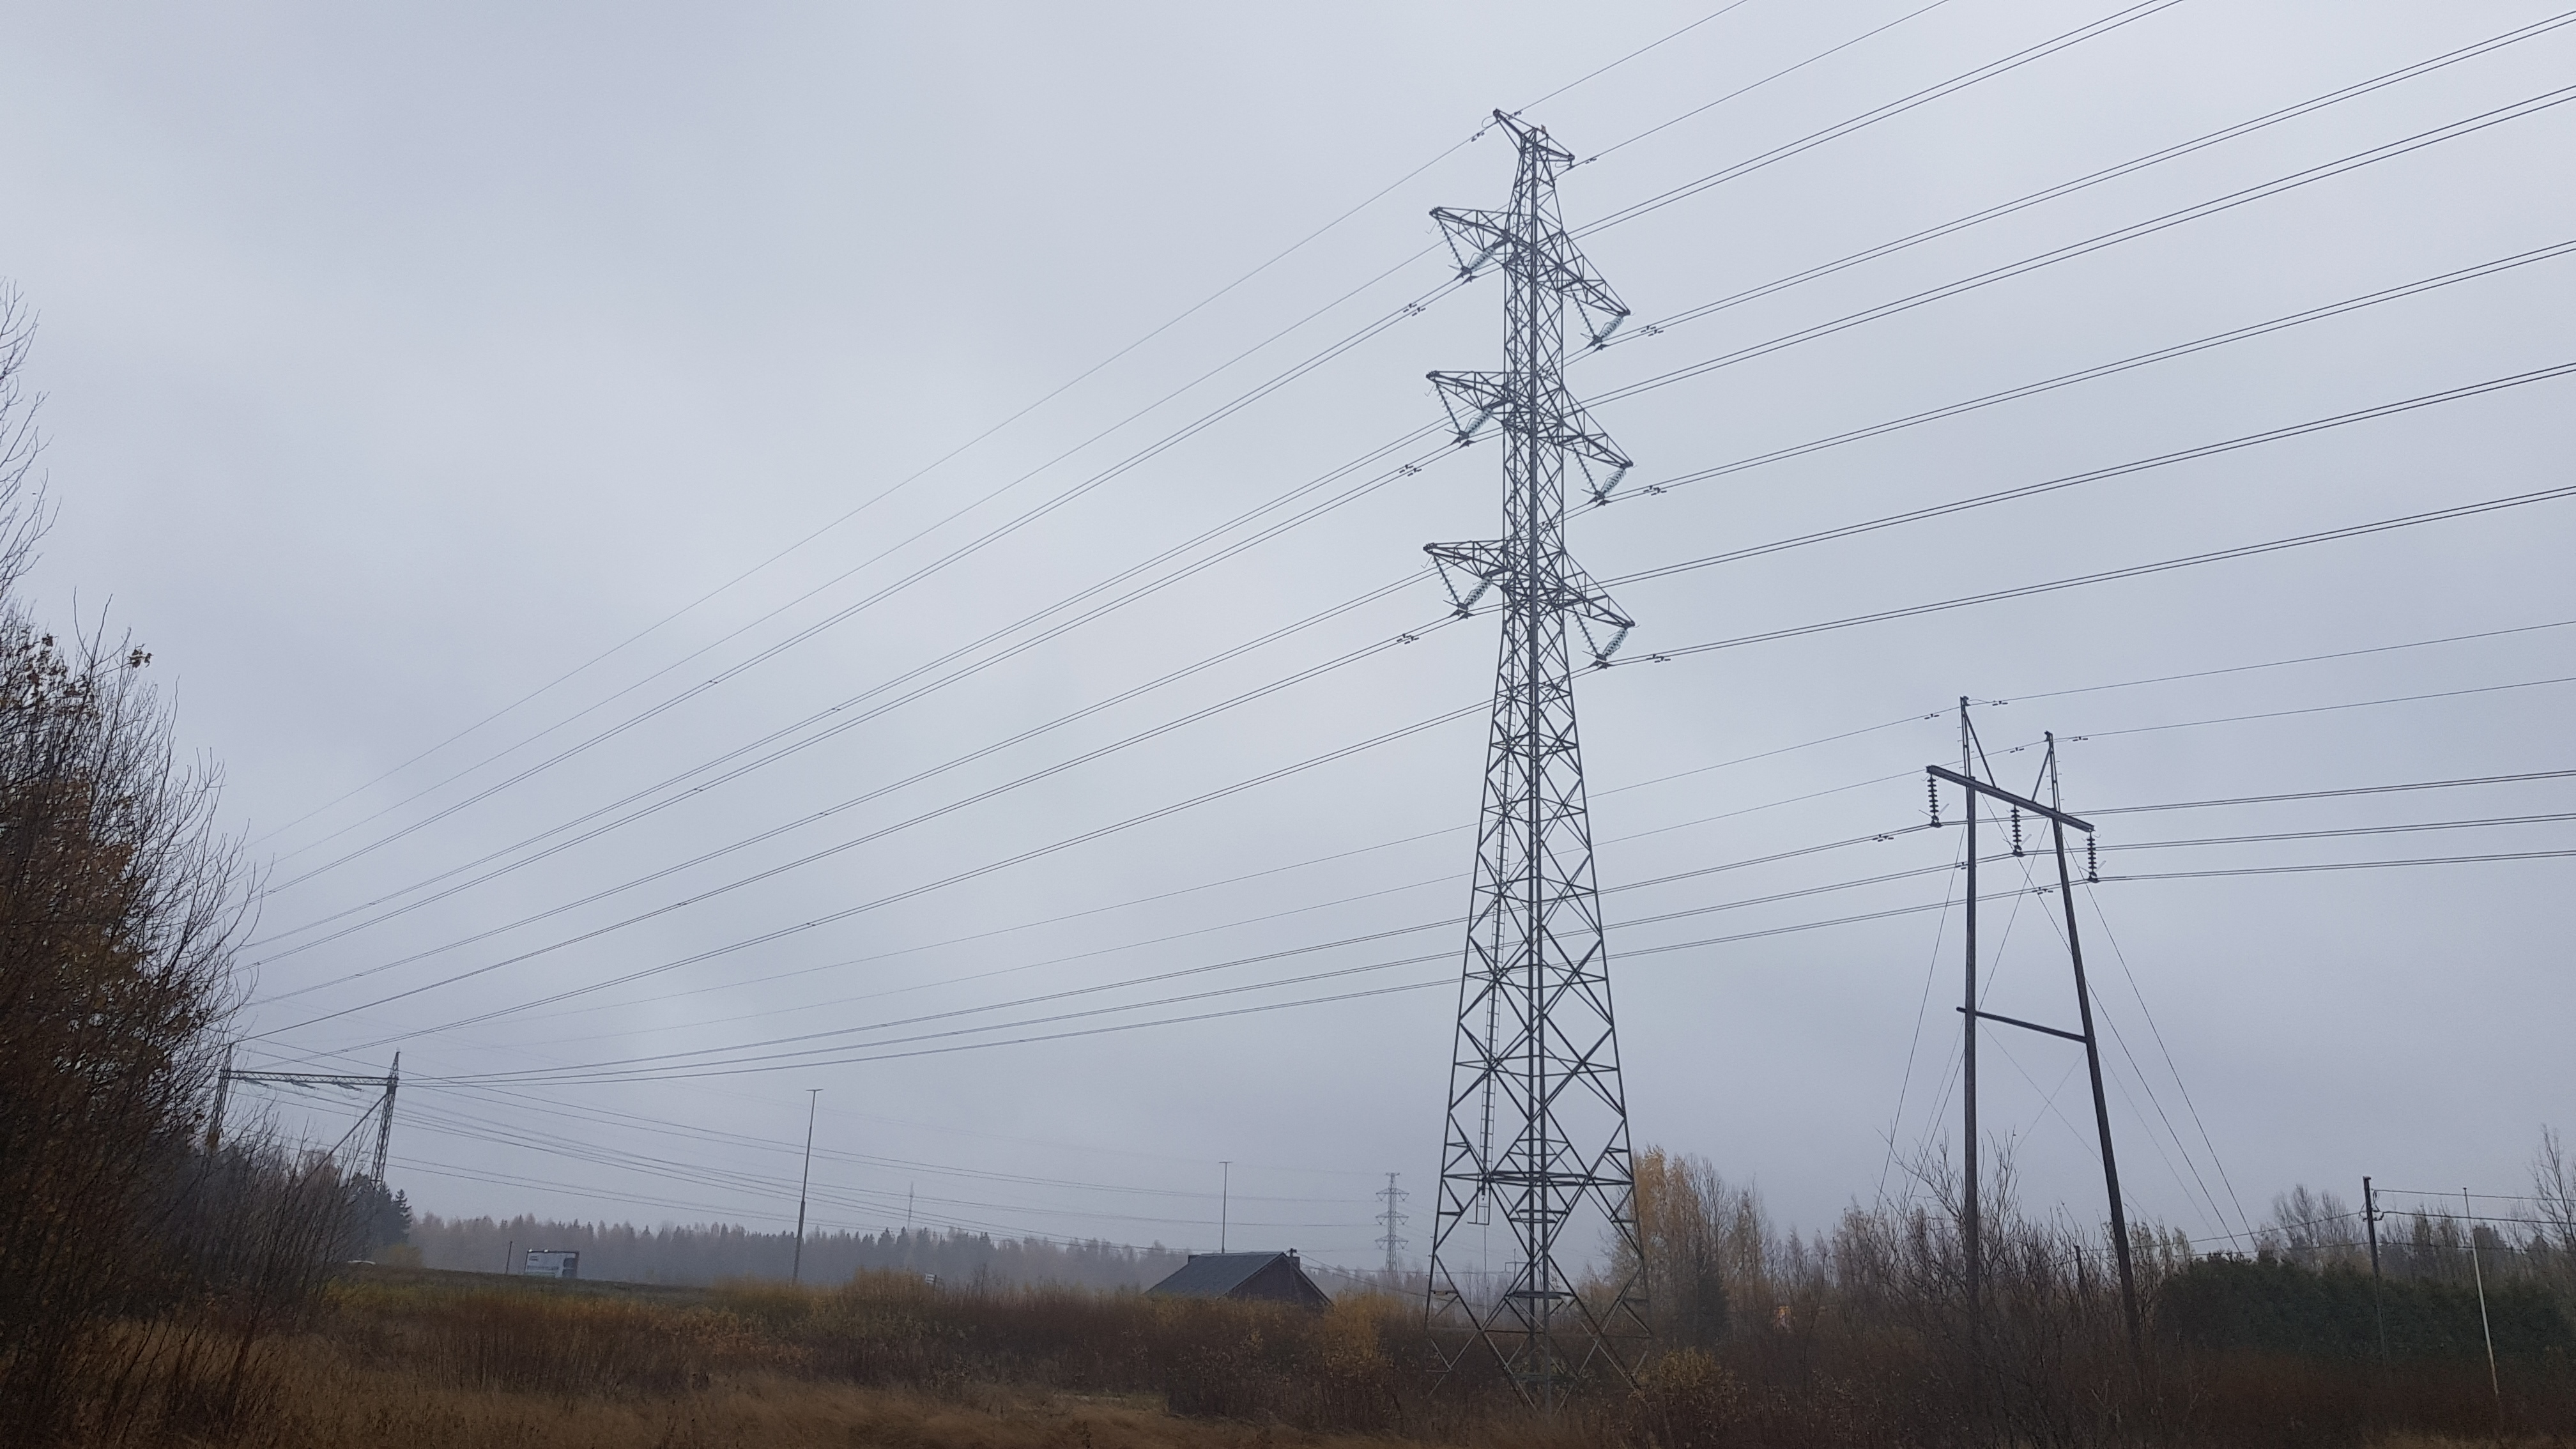
\includegraphics[keepaspectratio, width=0.94\paperwidth]{powerline_h.jpg}
\end{frame}

\begin{frame}{They come in all shapes}
\centering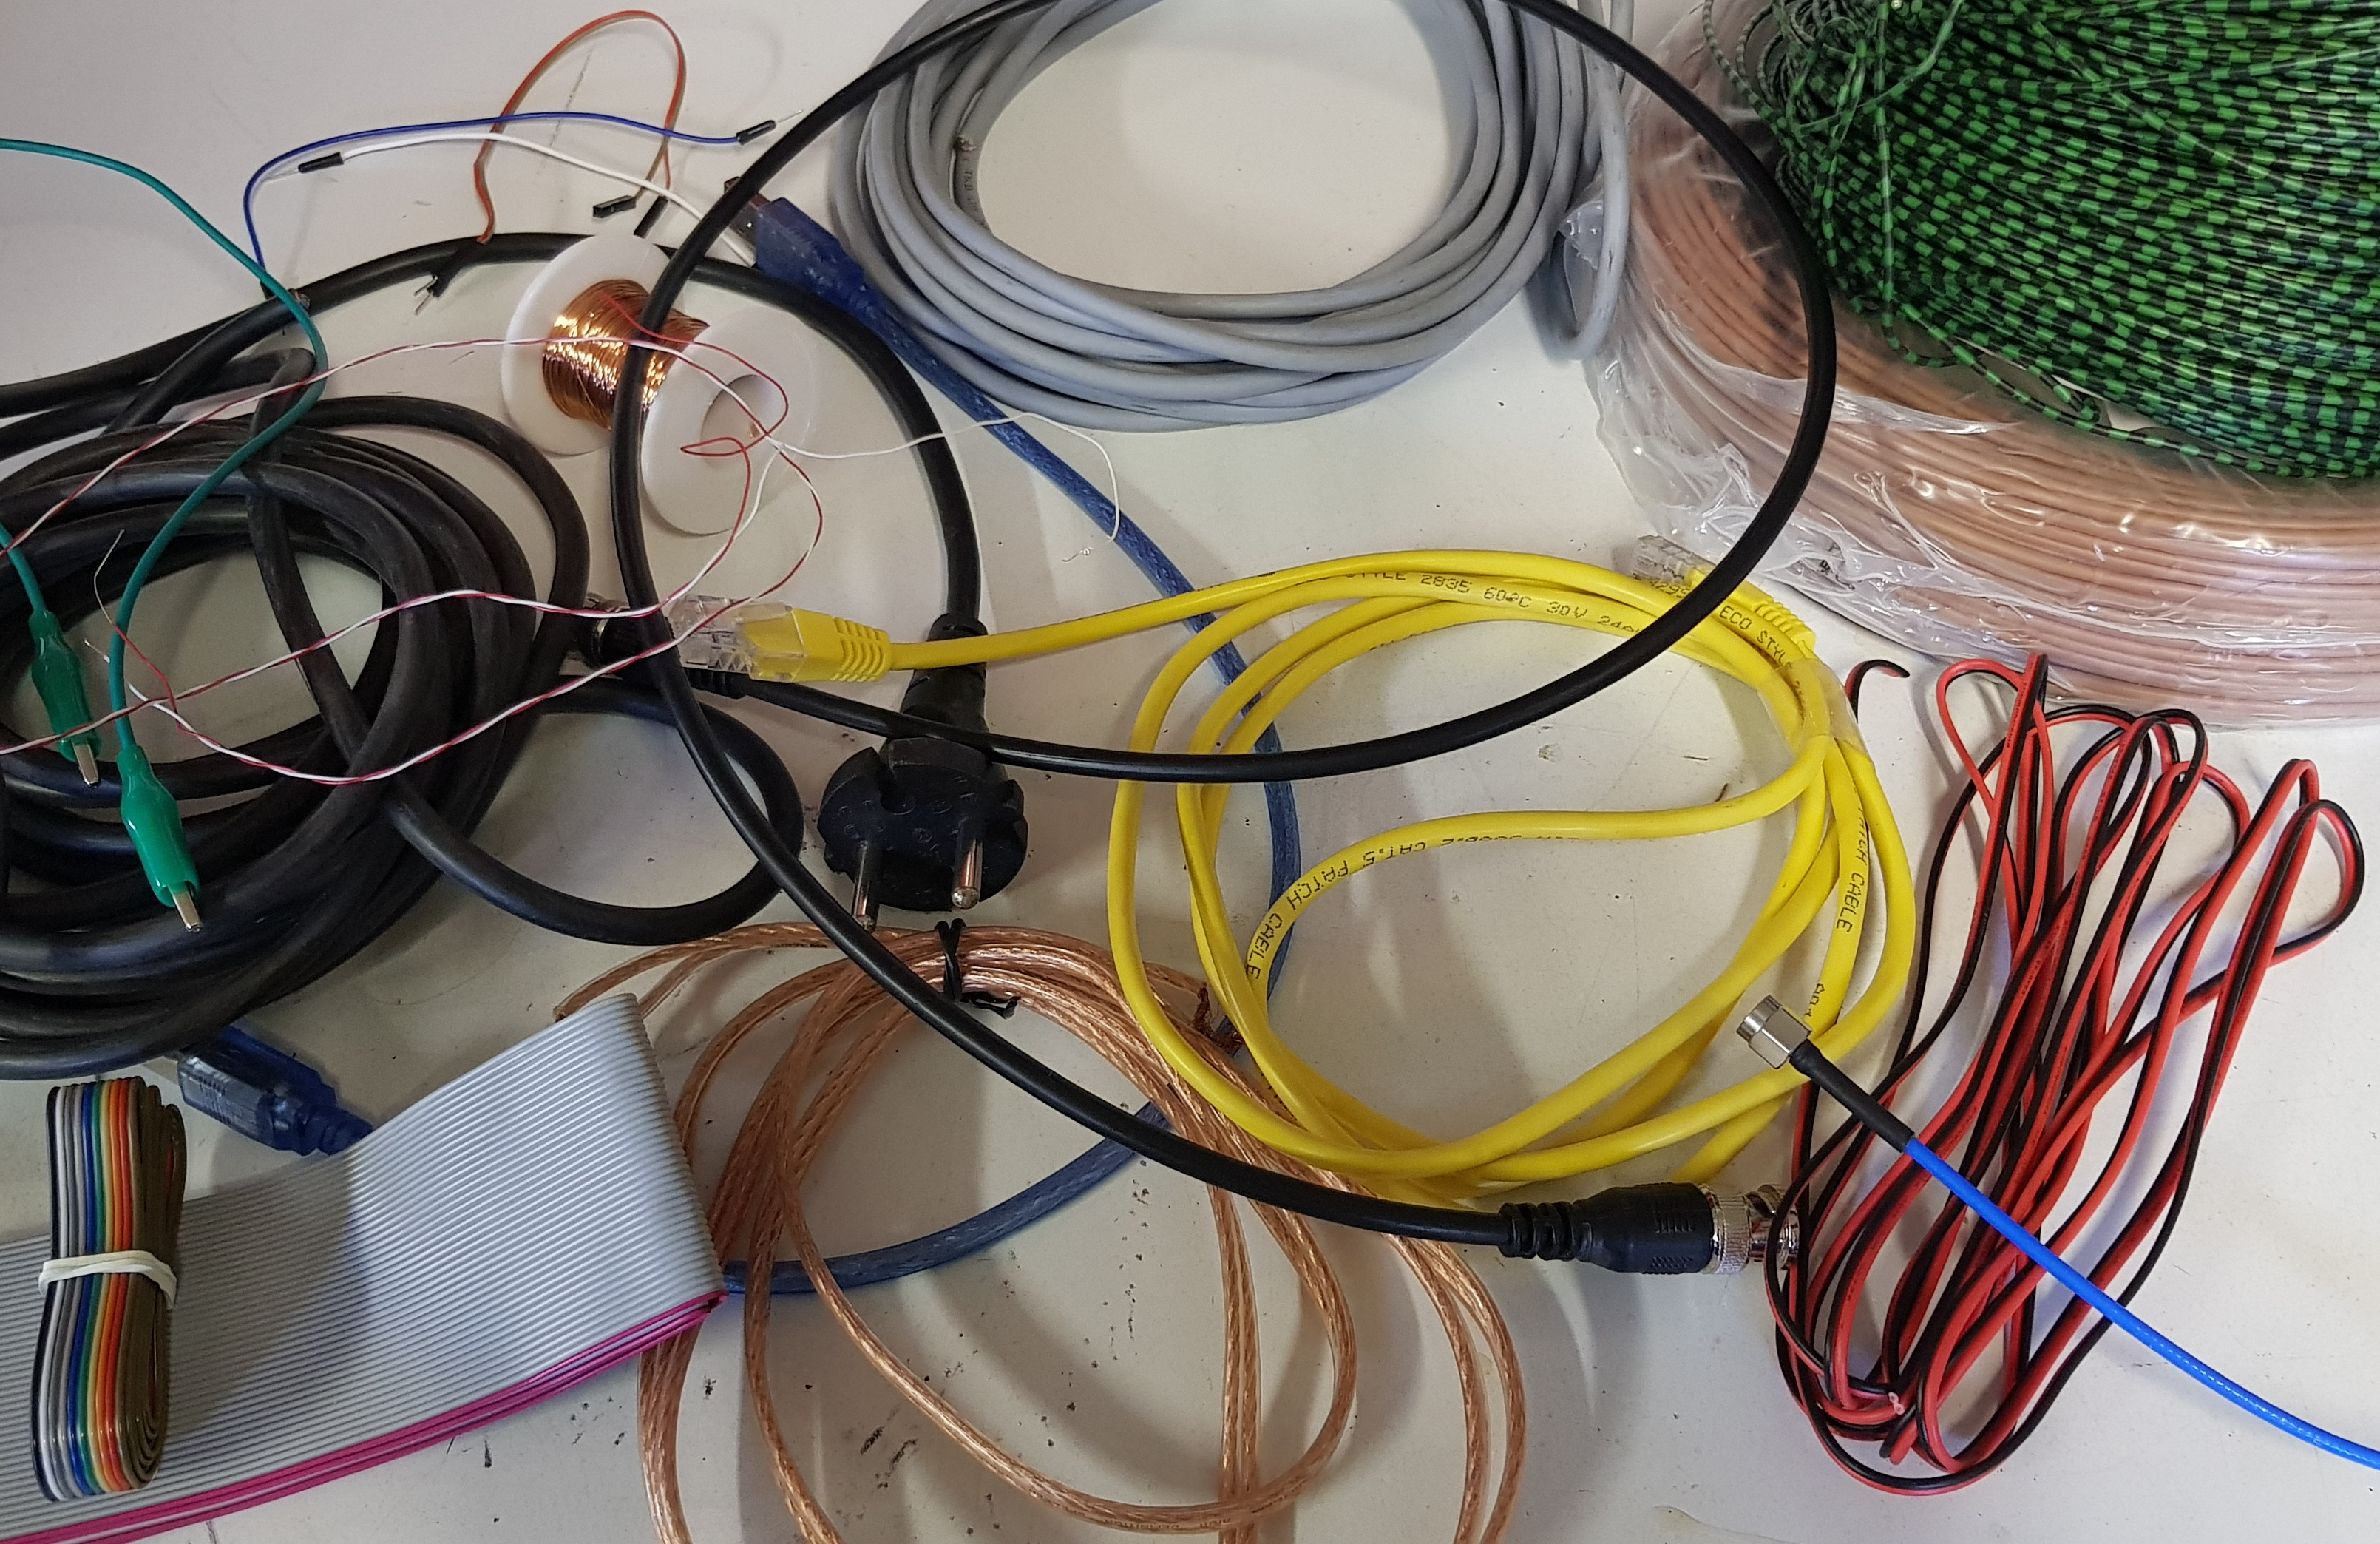
\includegraphics[keepaspectratio, width=0.88\paperwidth]{wires.jpg}
\end{frame}

\logo{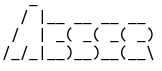
\includegraphics[scale=0.2]{logo_plain.png}}

\begin{frame}{Kinds of conductors}
 \begin{description}
  \setbeamertemplate{description item}[align left]
  \item[cable] multiple insulated wires within a jacket
  \item[\hyperlink{coaxial}{coaxial cable}] a cable where an inner conductor is surrounded by a conducting shield
  \item[flat cable] multiple insulated wires attached side by side so that they form a flat ribbon
  \item[PCB trace] A conductive path on a printed circuit board
  \item[\hyperlink{fatique}{stranded wire}] Number of small wires bundled or wrapped together for an enhanced flexibility
  \item[twisted pair] a cable construct where wire pairs are twisted together for a better electromagnetic compatibility
  \item[wire] a single conductor
 \end{description}
\end{frame}

\begin{frame}{What are the wires}
\begin{columns}
 \begin{column}{0.48\textwidth}
   \begin{itemize}
    \only<1->{\item Conductors?
	  \begin{circuitikz}
	    \draw (0,0) to[ short ] (2,0); 
	  \end{circuitikz}}    
    \only<2->{\item Resistors?
	  \scalebox{0.5}{\begin{circuitikz}
	    \draw (0,0) to[ european resistor ] (2,0); 
	  \end{circuitikz}}}
    \only<3->{\item Antenna?
	  \scalebox{0.3}{\begin{circuitikz}
            \node[antenna, xscale=-1] {};
	  \end{circuitikz}}}
    \only<4->{\item Capasitors?
	  \scalebox{0.3}{\begin{circuitikz}
	    \draw (0,0) to[ capacitor ] (2,0); 
	  \end{circuitikz}}}
    \only<5->{\item Inductors?
	  \scalebox{0.5}{\begin{circuitikz}
	    \draw (0,0) to[ cute inductor ] (2,0); 
	  \end{circuitikz}}}
    \only<6->{\item Clotheslines?}
   \end{itemize}
 \end{column}
 \begin{column}{0.48\textwidth}
  \tcbox[colframe=green!30!black, colback=green!30]{
    \only<1>{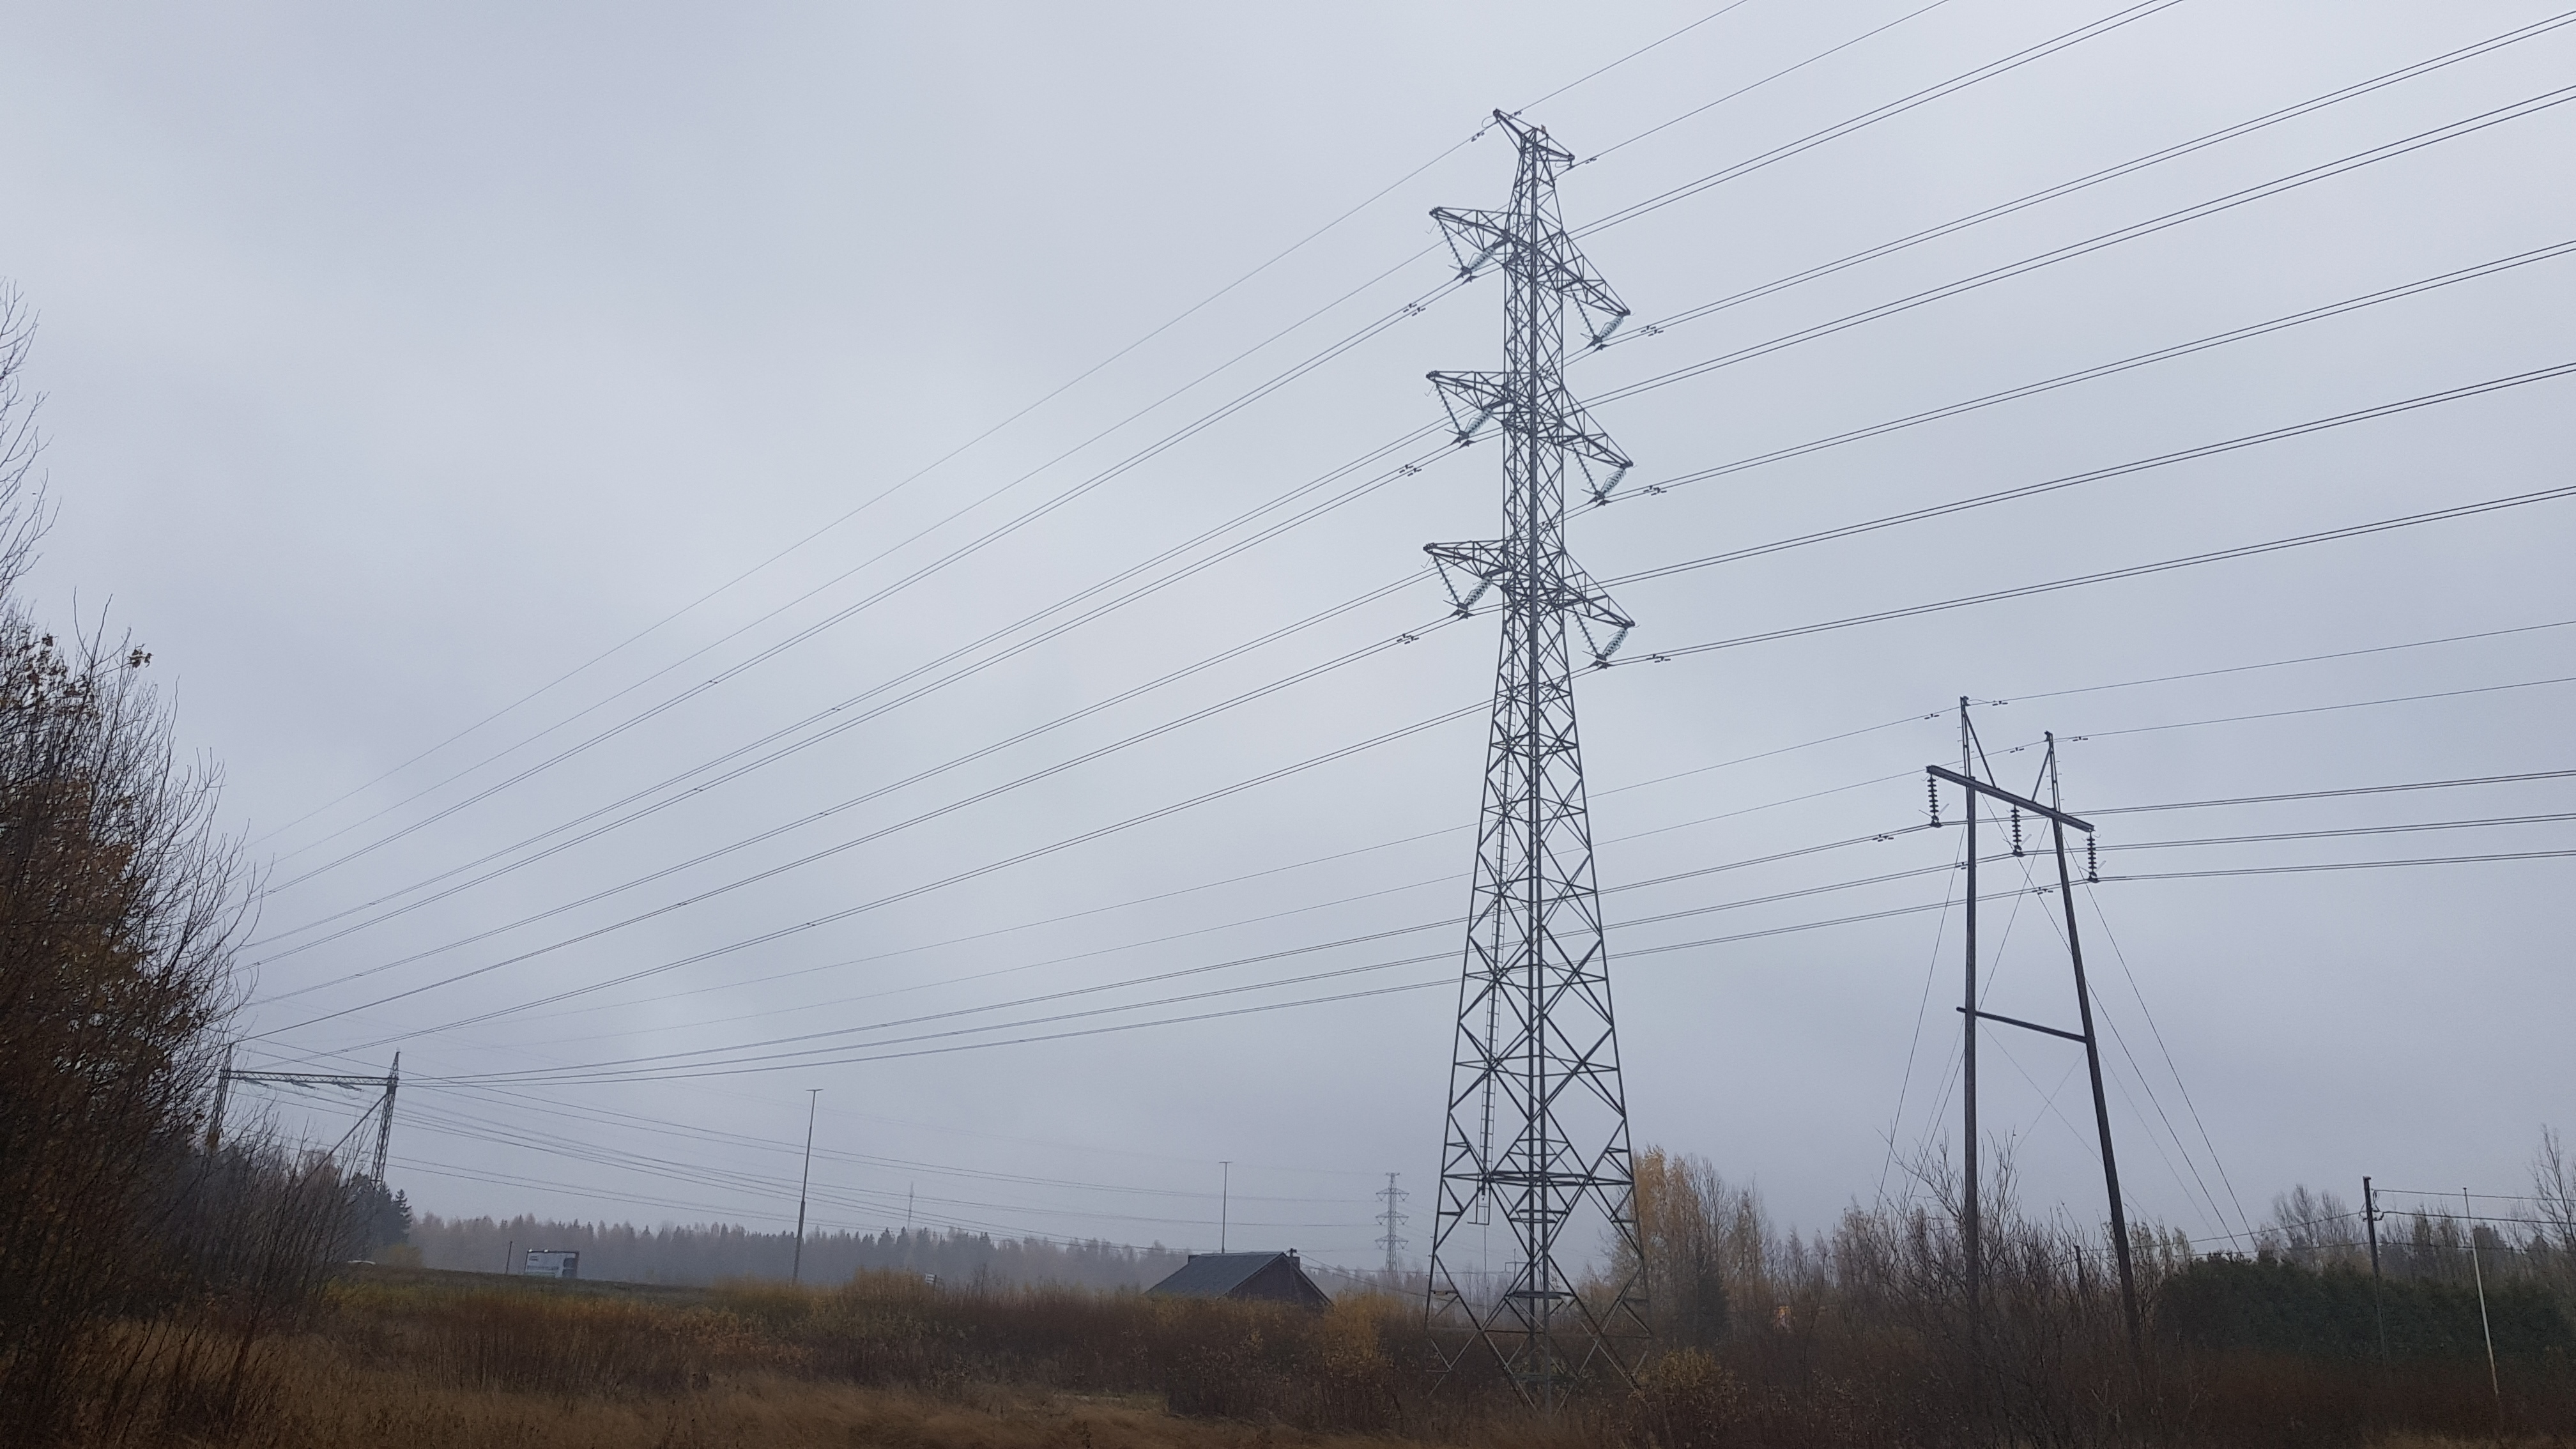
\includegraphics[width=0.75\linewidth]{powerline_h.jpg}
    }\only<2>{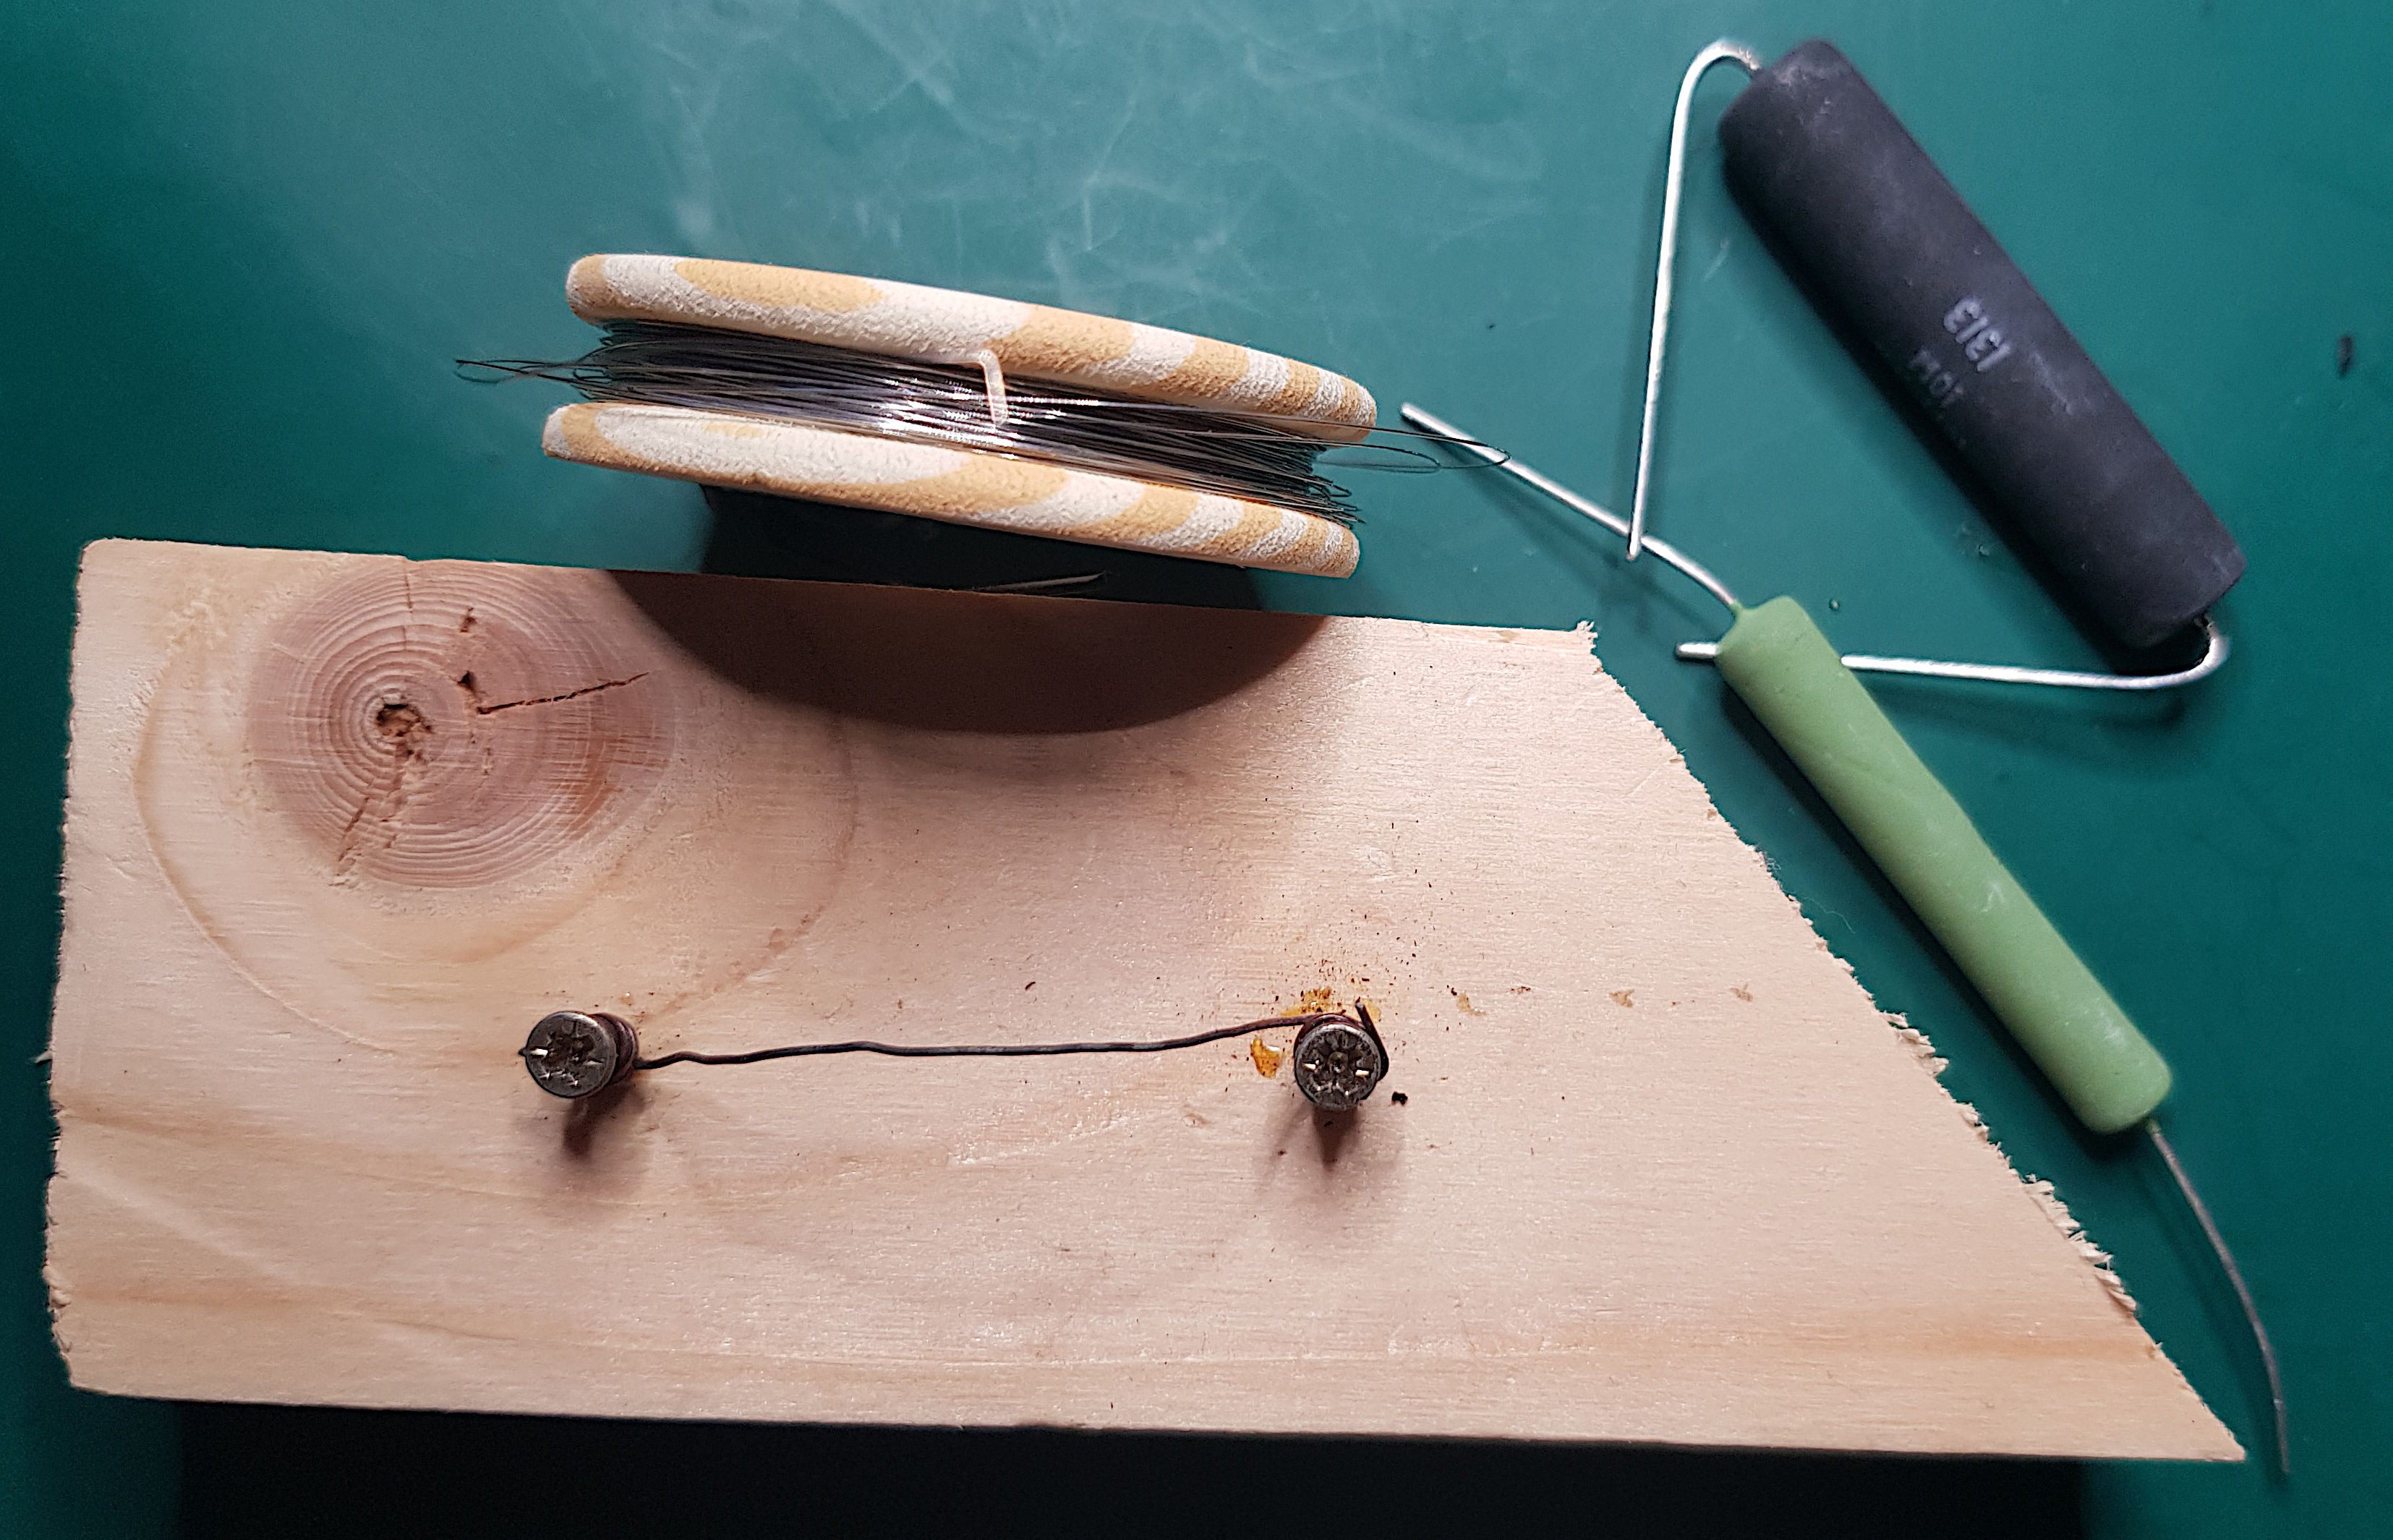
\includegraphics[width=0.75\linewidth]{resistor.jpg}
    }\only<3>{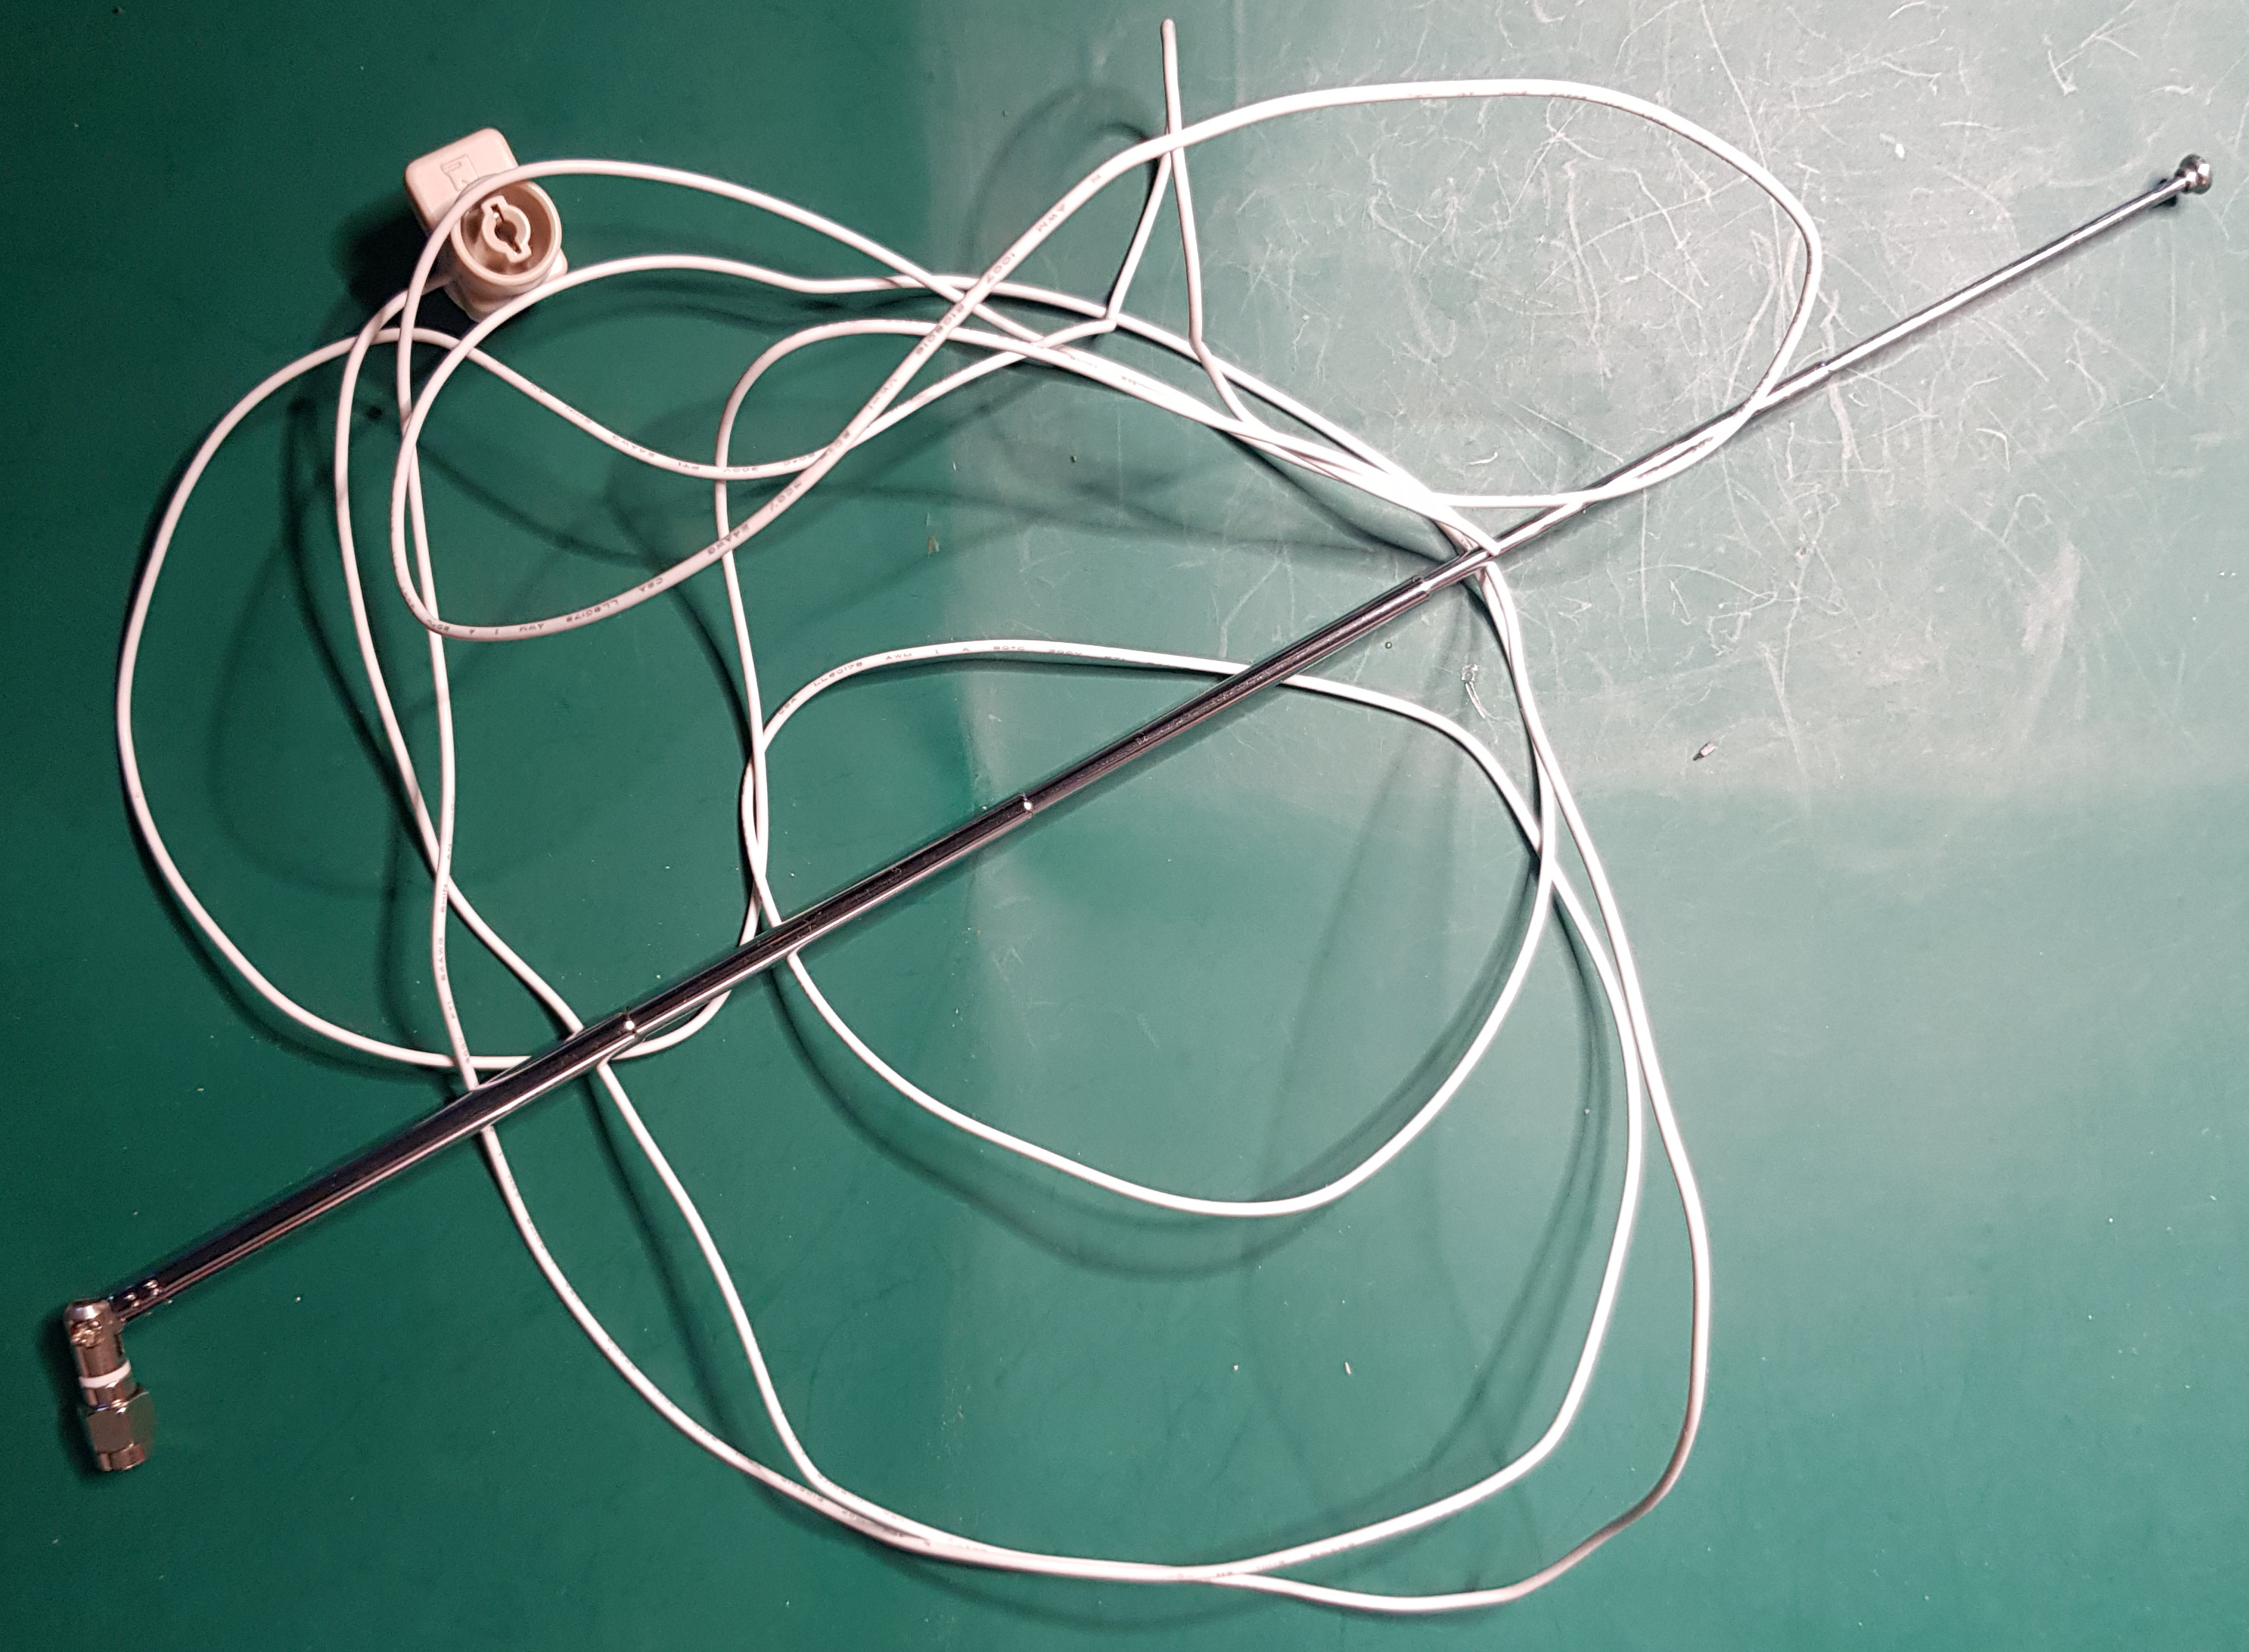
\includegraphics[width=0.75\linewidth]{antenna.jpg}
    }\only<4>{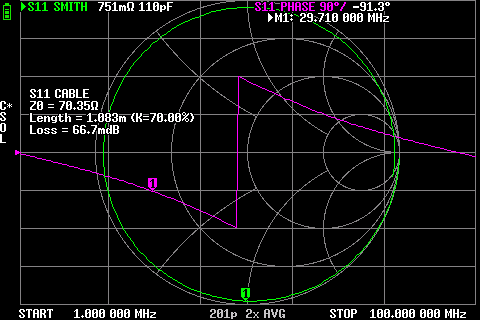
\includegraphics[width=0.75\linewidth]{CAP.png}
    }\only<5>{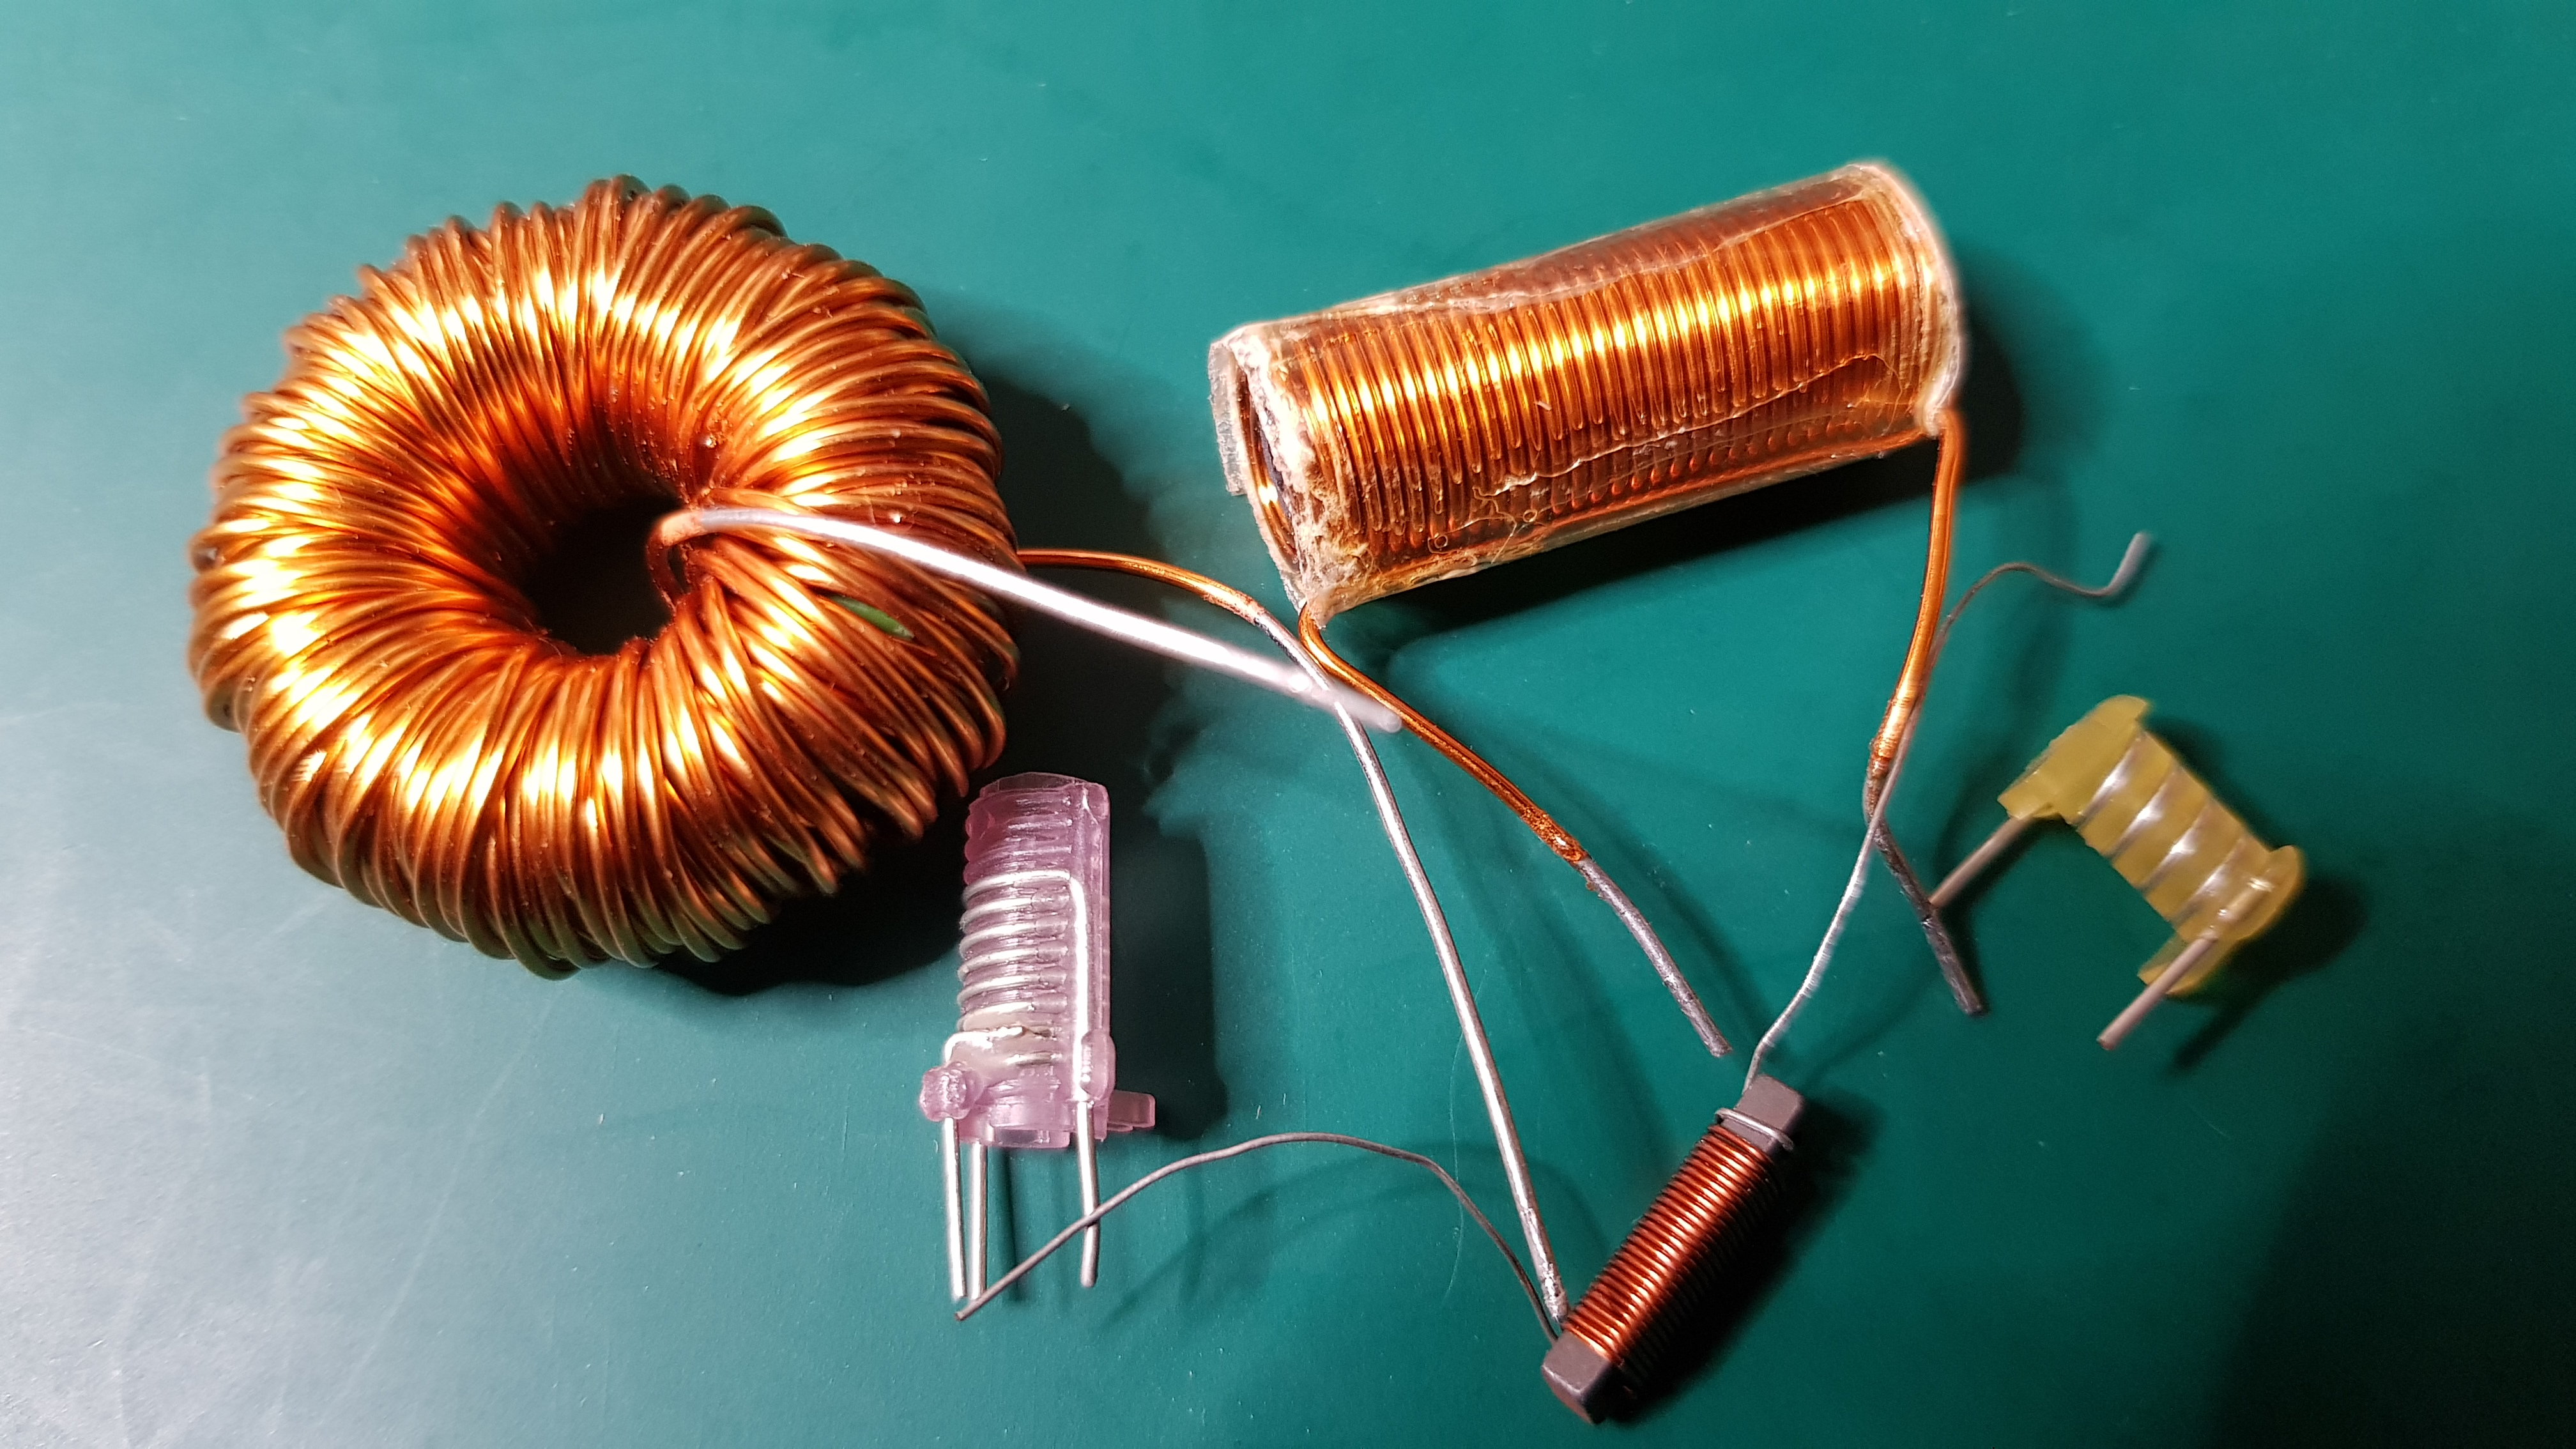
\includegraphics[width=0.75\linewidth]{inductors.jpg}
    }\only<6->{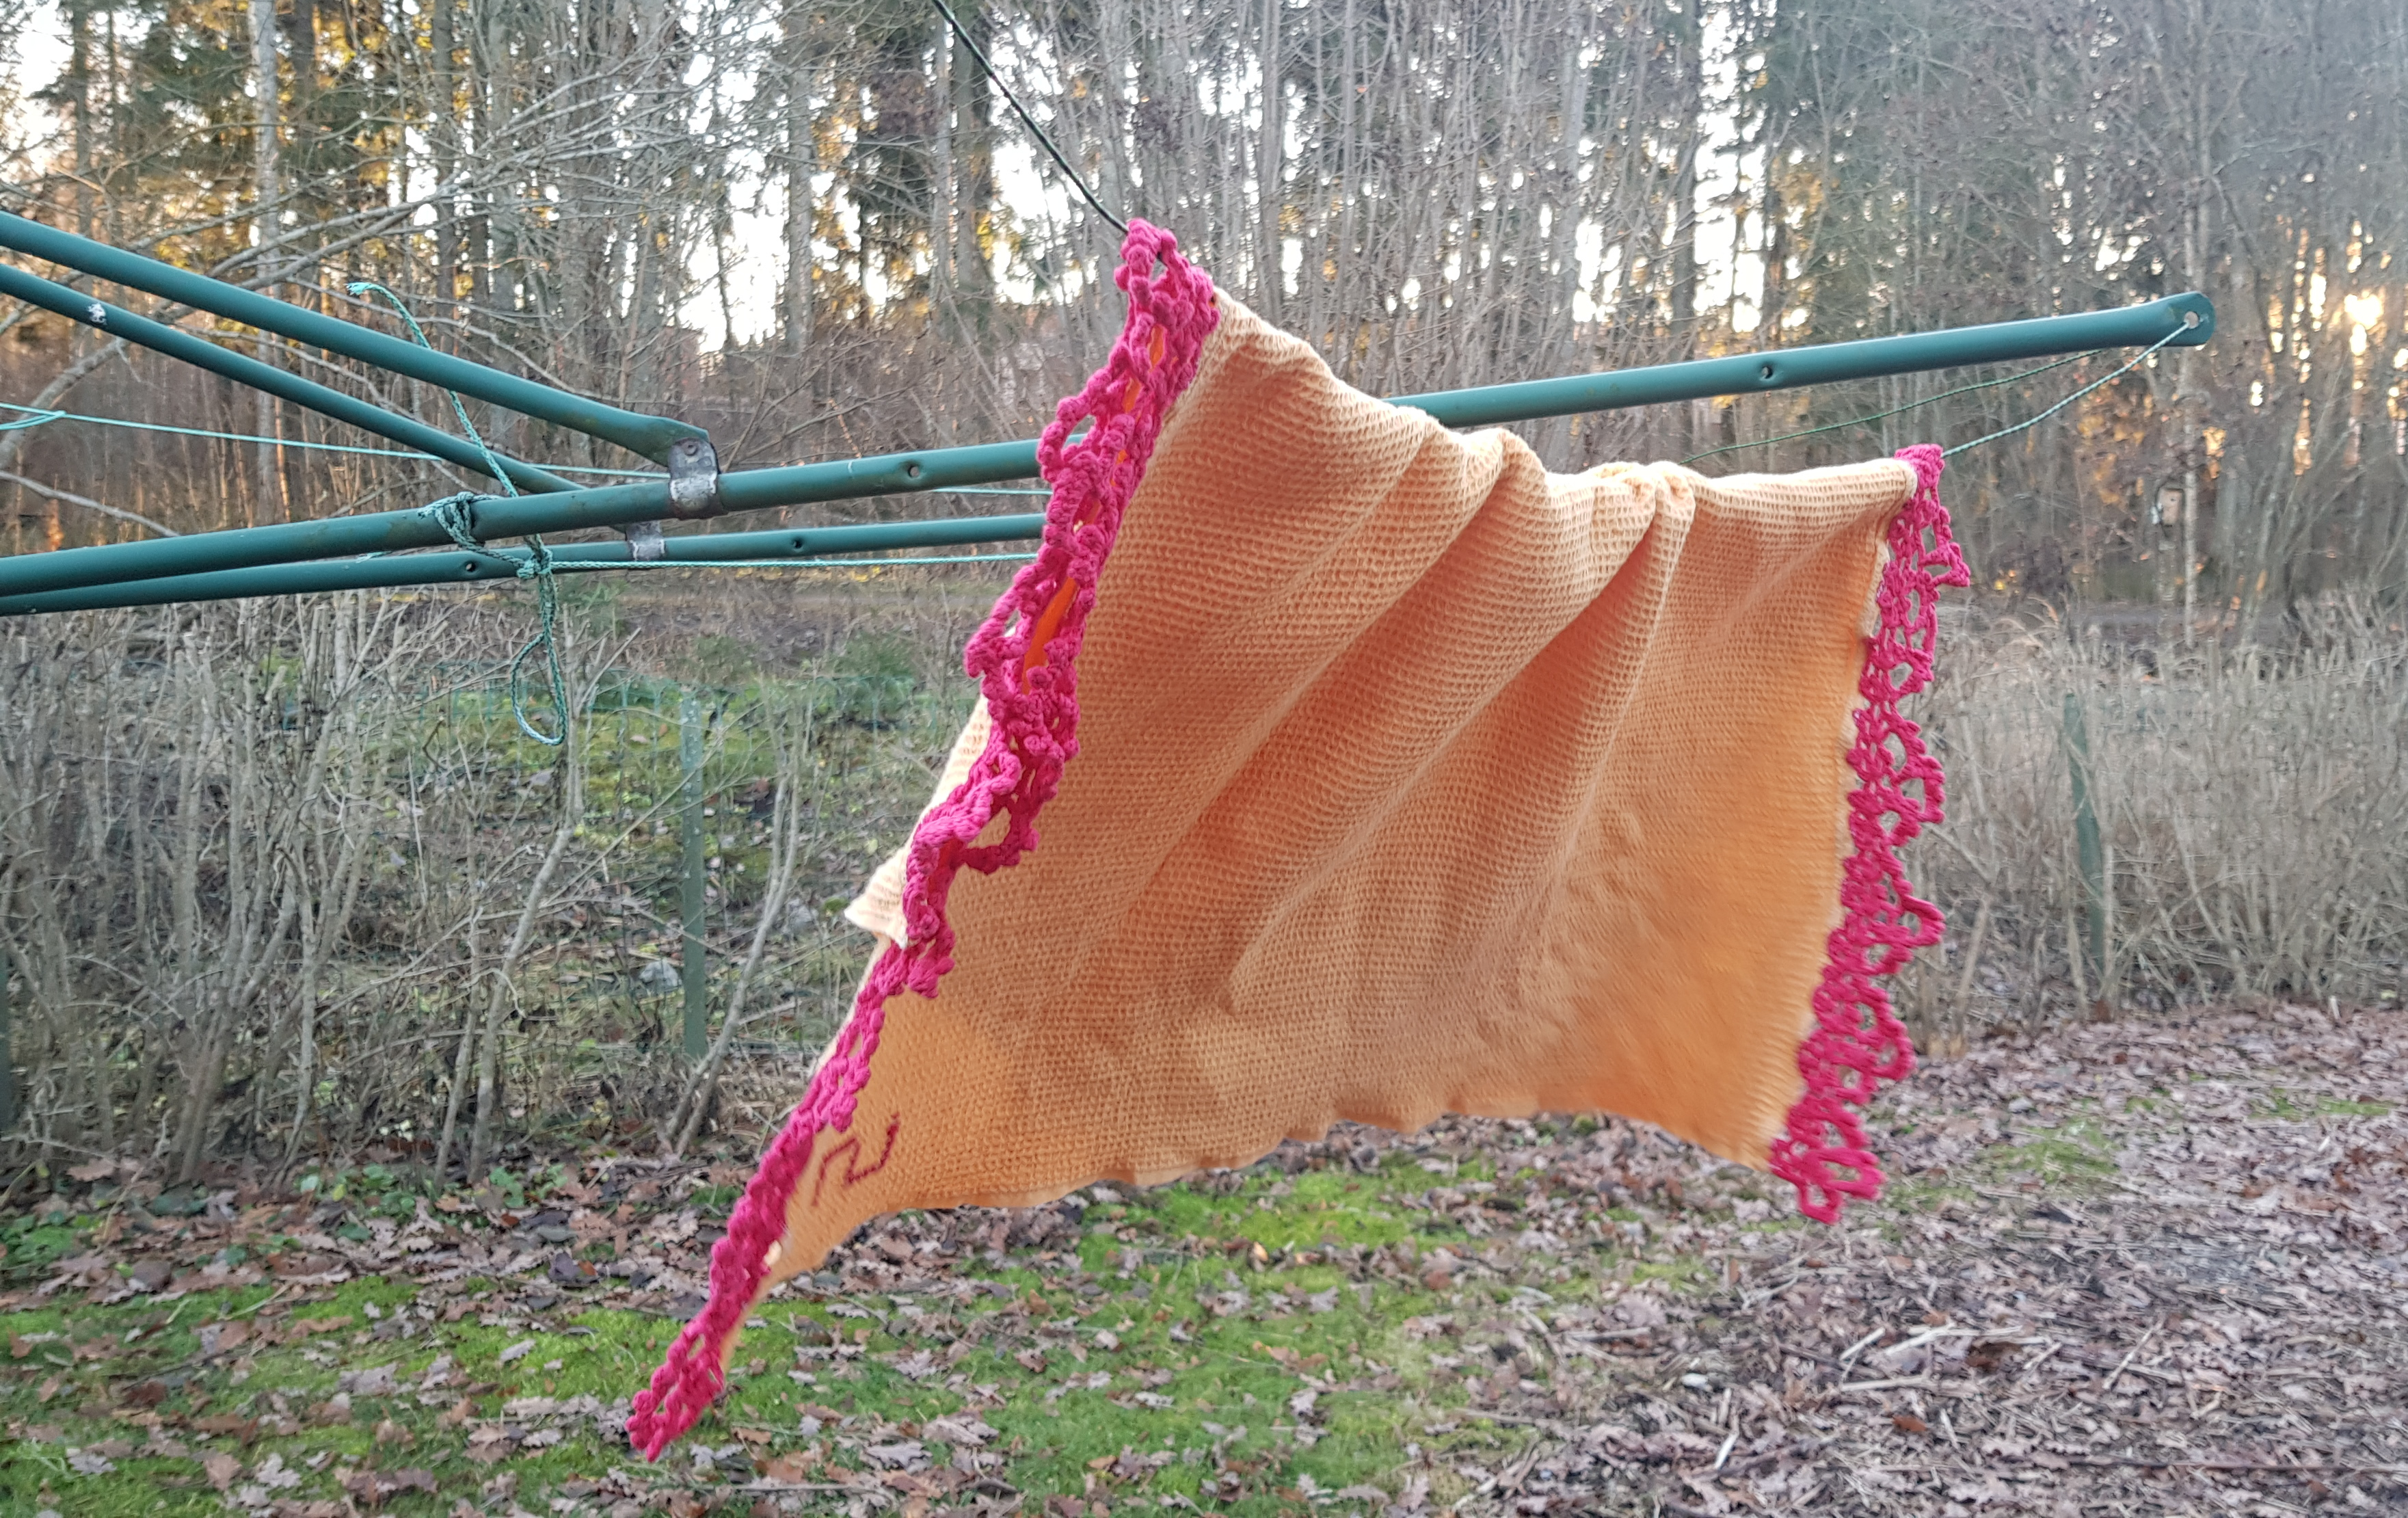
\includegraphics[width=0.75\linewidth]{clothesline.jpg}}
  }
  \only<1>{Charge carriers are transferred along the wires.}
  \only<2>{Some energy is dissipated as heat unless superconductors.}
  \only<3>{Unshielded wires can be used to transmit and receive electromagnetic radiation.}
  \only<4>{Wires store tiny charges and their parasitic capacitance can be seen in many sensitive, high-frequency applications.}
  \only<5>{A magnetic field forms around a conducting wire and it stores some energy.}
  \only<6->{The mechanical strength of a wire can be used for various applications.}
 \end{column}
\end{columns}
\vspace{20px}
\only<7>{\centering\huge\color{purple} All that and a lot more!}
\only<8->{One may consider many linear components special wires in special configuration emphasizing some of the intended properties.}
\end{frame}

\begin{frame}{Connectors}
\begin{columns}
  \begin{column}{0.48\textwidth}
   \begin{itemize}
    \item Strong, solderless and detachable joints
   \end{itemize}
  \end{column}
  \begin{column}{0.48\textwidth}
   \tcbox[colframe=green!30!black, colback=green!30]{
    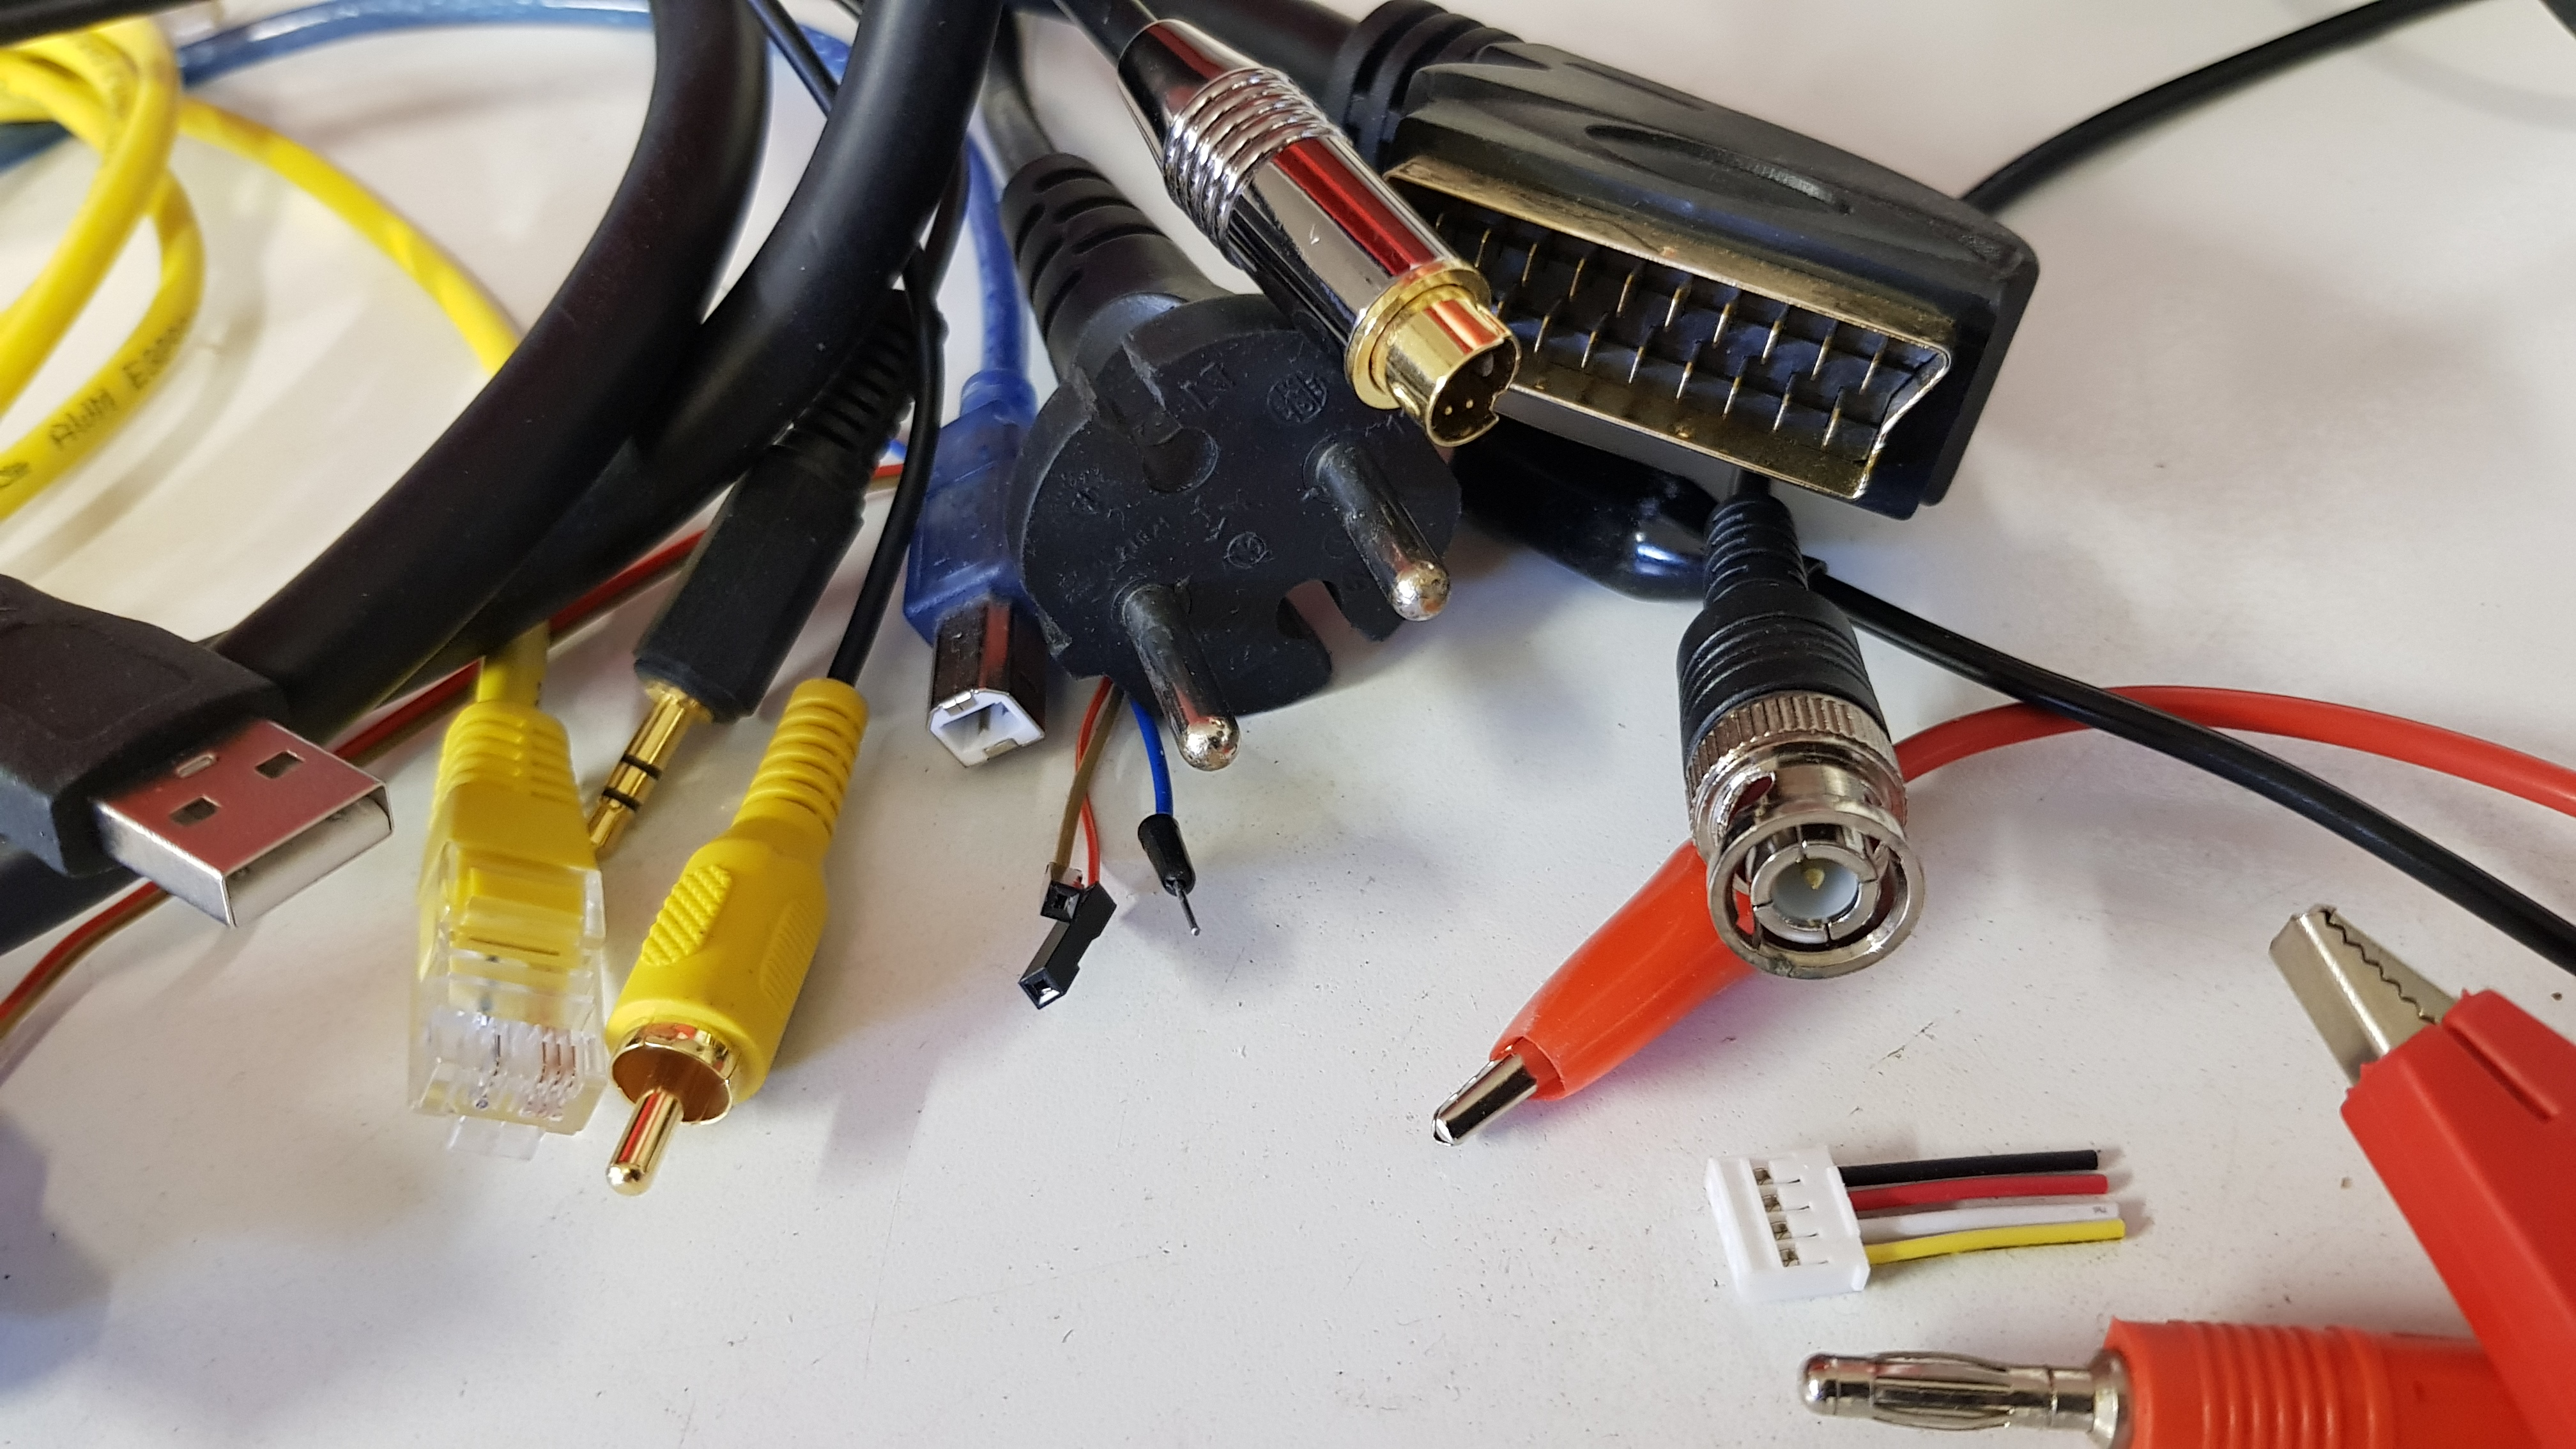
\includegraphics[width=0.65\linewidth]{connectors.jpg}
  } 
  \end{column}
\end{columns}
\end{frame}

\begin{frame}[label=fatique]{Metal fatique}
 \begin{itemize}
  \item Metal wires and their connection points especially, are prune for fractures when bended
  \item Stranded wires are more resistant against the metal fatigue than typical solid wires
  \item \textbf{Vibrating or moving wires shall not be soldered}
  \item Clamp connectors are more resistant
  \item A connector can be followed by a sleeve for some extra support
 \end{itemize}
\end{frame}

\section{Physical properties}

\begin{frame}{Some of their properties include}
 \begin{itemize}
  \item Temperature range for operation ($\SI{}{\kelvin}$ interval)
  \item Elasticity
  \item Color
  \item UV resistance, durability
  \item Length ($\SI{}{\meter}$)
   \begin{itemize}
    \item Mass ($\SI{}{\kilo\gram}$)
    \item Resistance ($\SI{}{\ohm}$), conductance ($\SI{}{\siemens}$)
    \item \hyperlink{impedance}{Impedance} ($\SI{}{\ohm}$), admittance ($\SI{}{\siemens}$)
    \item Price
   \end{itemize}
  \item Cross-sectional area ($\SI{}{\meter^2}$)~\cite{iec2004}
 \end{itemize}
\end{frame}

\begin{frame}[label=impedance]{Impedance}
\begin{columns}
  \begin{column}{0.58\textwidth}
   \begin{itemize}
    \item Impedance is the total opposition to alternating current
    \item Unit is ohm ($\SI{}{\ohm}$)
    \item Resistance means energy loss as heat
    \item No energy is lost through the reactance
    \item Reactance consists of capacitive ($X_C$) and inductive ($X_L$) reactance
     \begin{itemize}
      \item inductive reactance ($X > 0$)
      \item purely resistative ($X > 0$)
      \item capacitative reactance ($X < 0$)
     \end{itemize}
   \end{itemize}
  \end{column}
  \begin{column}{0.38\textwidth}
    \begin{block}{$Z = R + jX$}
        $R$ is the resistance \\
        $X$ is the reactance\footnote{Please notice the imaginary symbol of $j = \sqrt{-1}$ in place of the typical $i$. This is to avoid confusion with the current symbol.}
    \end{block}
  \end{column}
\end{columns}
\end{frame}

\begin{frame}{Skin effect}
 \begin{tikzpicture}[remember picture,overlay]
  \filldraw[xshift=0.85\linewidth, yshift=-3.3cm, inner color=white, outer color=blue] (0,0) circle (1.2);
  \draw[xshift=0.85\linewidth, yshift=-3.3cm](0,0) circle (0.9);
 \end{tikzpicture}
 \begin{itemize}
  \item Current dencity of an AC tends to form an exponentially decreasing gradient towards the depth of the conductor
  \item Skin depth ($\delta$) represents the depth where the current density drops below $e^{-1} \approx 37\%$
  \item
    $\delta = \frac{1}{\sqrt{\pi f \mu  \sigma}}$, where
    \begin{description}
      \setbeamertemplate{description item}[align left]
      \item[$f$] the frequency of the current
      \item[$\mu$] the permeability of the material
      \item[$\sigma$] conductivity of the material
    \end{description}
  \item Makes the signal losses frequency dependent
 \end{itemize}
\end{frame}

\begin{frame}{Smith diagram}
\begin{columns}
 \begin{column}{0.58\textwidth}
  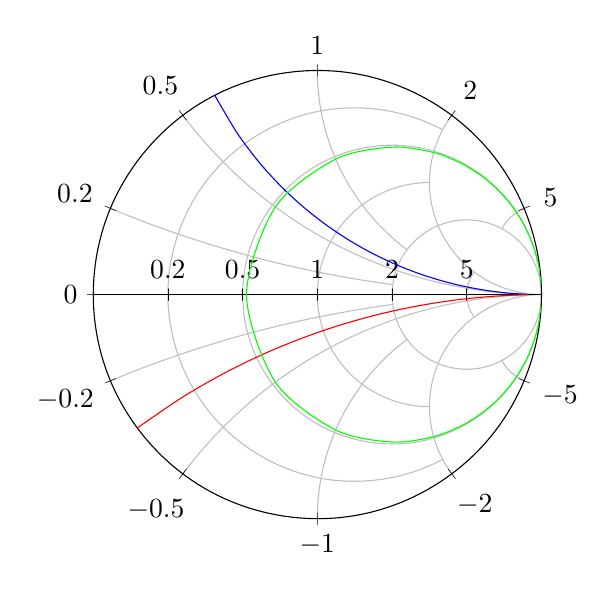
\begin{tikzpicture}
    \begin{smithchart}[samples=201, line cap=round, smooth]
      \addplot[domain=0:30, color=blue] (x,0.61);
      \addplot+[no marks, domain=0:30, color=red] (x,-0.33);
      \addplot+[no marks, domain=-50:50, color=green](0.52,x);
    \end{smithchart}
  \end{tikzpicture}
 \end{column}
 \begin{column}{0.5\textwidth}\small
 {\color{green}Constant resistance ($0.52$)}

 {\color{blue}Constant inductive reactance ($0.61$)}

 {\color{red}Constant capacitive reactance ($-0.33$)}
 \end{column}
\end{columns}
\end{frame}

\section{Speed of electricity}

\begin{frame}{Speed of electricity}
\begin{itemize}
 \item Electronic signals propagate approximately at $c/2$ along the PCB traces~\cite[p. 8--9]{horowitz2020art}
 \item Matching trace lengths to keep signals in sync
 \begin{itemize}
  \item $\SI{25}{\pico\second}$ tolerance between signal requires matching $<\SI{4}{\milli\meter}$
  \item DDM memory traces may need matching in length to $\SI{0.5}{\milli\meter}$!\\
        \tcbox[colframe=green!30!black, colback=green!30]{
          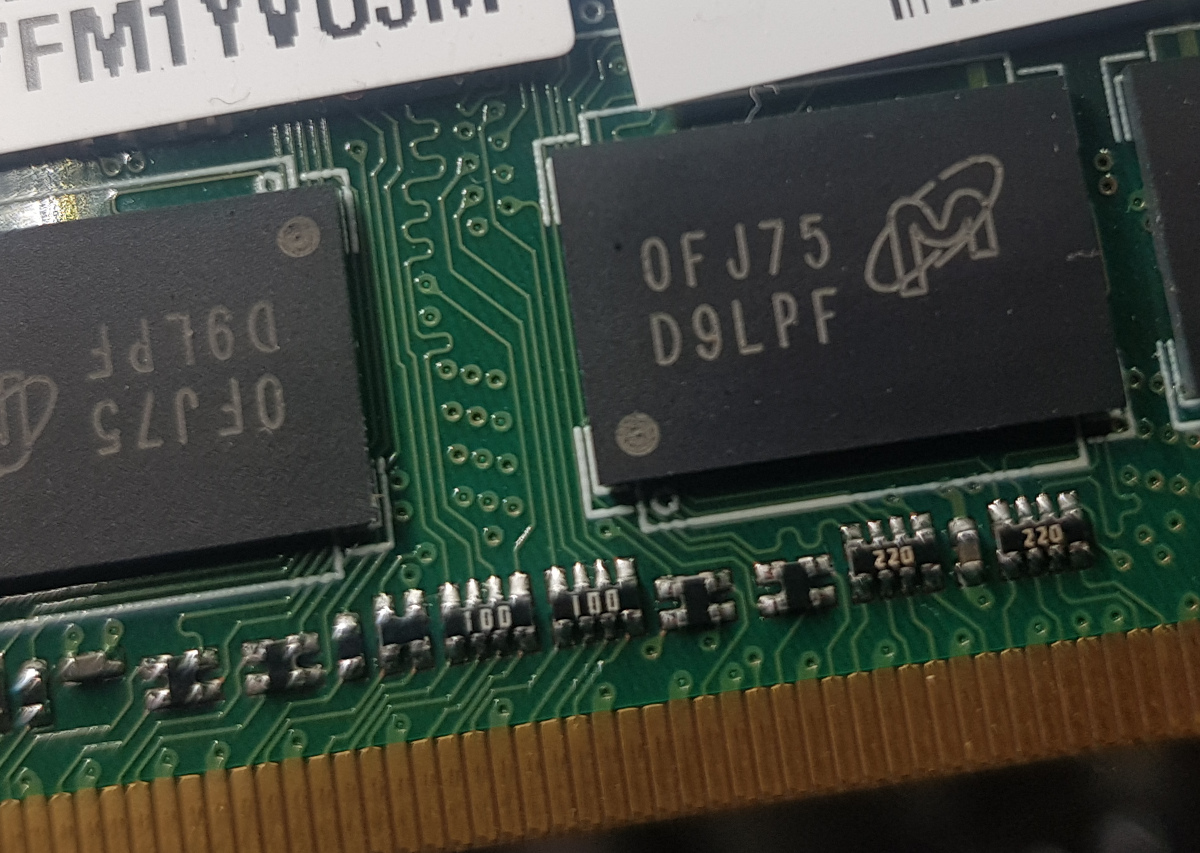
\includegraphics[width=0.45\linewidth]{trace_length.jpg}
        }
 \end{itemize}
\end{itemize}
\end{frame}

\begin{frame}{Speed of electrons}
\begin{itemize}
 \item The average movement of the charged particles is called drift velocity
 \begin{itemize}
  \item Proportional to current
  \item Proportional to the strength of the electric field in resistive materials
 \end{itemize}
 \item Electrons move randomly in the absence of an electric field (drift velocity is 0)
 \item The drift velocity in a $\SI{2}{\centi\meter}$ diameter copper wire in
       $\SI{1}{\ampere}$ current $\approx\SI{8}{\centi\meter}$ per hour~\cite{wiki:Speed_of_electricity}
 \item Back and forth movement in alternating current (no net movement)
 \begin{itemize}
  \item Within few micrometers
 \end{itemize}
\end{itemize}

\end{frame}

\begin{frame}[t]{Signal propagation}{}
\only<1>{{\footnotesize Varitasium introduced an interesting setup to demonstrate how the signal propagates within an electrical circuit~\cite{veritasium2021}.
 Here, we represent a somewhat simplified setup along the same idea.}}

How long does it take for the signal to reach our voltmeter once we press the button?

\begin{circuitikz}
  \draw (0,0)
  to[short] (0,2)
  to[short, l_=${l_{left} = \SI{1}{\second}\times c}$~\footnote{$\SI{1}{\second}\times c=\SI{299 792 458}{\meter}$}] (3,2)
  to[voltmeter] (6,2)
  to[short, l_=${l_{right} = \SI{1}{\second}\times c}$] (10,2)
  to[short] (10,0)
  to[push button] (3,0)
  (2,0) to[battery, v_={~}] (3,0)
  to[short] (0,0);
  \draw[B] (10,0) -- node[right=5pt] {$\SI{1}{\meter}$ apart} (10,2);
\end{circuitikz}
\only<2->{
 \begin{enumerate}[A.]
  \item<2-> \only<5>{\color{red}}$\approx \SI{1}{\second}$
    \only<2>{(travel half circuit from switch to the voltmeter)}
    \only<5>{\tiny\color{black} The full voltage will be reached as the current completes the half circuit but\ldots}
  \item<3-> \only<5>{\color{red}}$\approx \SI{2}{\second}$
    \only<3>{(complete the circuit back to the battery)}
  \item<4-> \only<5>{\color{green}}$\frac{1}{c}$
    \only<4>{(reach the parallel wire over the gap)}
    \only<5>{\tiny\color{black} We'll induce a low voltage to the parallel wire almost immediately.}
 \end{enumerate}
}
\end{frame}

\section{Transmission lines}

\begin{frame}{Transmission lines}
\begin{circuitikz}[scale=1.0]
   \draw
	(0,0) to [short, o-] (1,0)
	(1,0) to [transmission line] (3,0)
	(3,0) to [short, -o] (4,0);
\end{circuitikz}
\begin{itemize}
 \item Transmit power from source to load
 \item Theory becomes important as the length of the wire exceeds $\frac{\lambda}{20}$
 \item An open wire acts like a short circuit when its length is $\frac{\lambda}{4}$ (or its odd multiple)!
 \item Transmissions lines behave capacitively on low frequencies
\end{itemize}
\end{frame}


\begin{frame}[t]{Transmission lines}
\begin{circuitikz}[scale=0.4, transform shape]
  \draw
    (0,0) to [short, o-] (1,0)
    (19,0) to [short] (0,0)
    (21,0) to [short, -o] (23,0)
    (21,5) to [short, -o] (23,5)
    (0,5) to [short, o-] (1,5)
    ;
  \draw
    (1,5) to [L, l=$L_1$] (3,5)
    (7,5) to [L, l=$L_2$] (9,5)
    ;

  \draw[visible on=<1>]
    (3,5) to [R, l=$R_{s1}$] (7,5)

    (7,0) to [short] (7,1)
    (6,1) to [short] (8,1)
    (6,1) to [C, l=$C_1$] (6,4)
    (8,1) to [R, l=$R_{g1}$] (8,4)
    (6,4) to [short] (8,4)
    (7,5) to [short] (7,4)

    (9,5) to [R, l=$R_{s2}$] (13,5)

    (13,0) to [short] (13,1)
    (12,1) to [short] (14,1)
    (12,1) to [C, l=$C_2$] (12,4)
    (14,1) to [R, l=$R_{g2}$] (14,4)
    (12,4) to [short] (14,4)
    (13,5) to [short] (13,4)
    ;
  \draw[visible on=<2>]
    (3,5) to [short] (7,5)
    (7,0) to [C, l=$C_1$] (7,5)
    (9,5) to [short] (13,5)
    (13,0) to [C, l=$C_2$] (13,5)
    ;
  \draw[color=gray, visible on=<1>]
    (13,5) to [L, l=$L_n$] (15,5)
    (15,5) to [R, l=$R_{sn}$] (19,5)

    (19,0) to [short] (19,1)
    (18,1) to [short] (20,1)
    (18,1) to [C, l=$C_n$] (18,4)
    (20,1) to [R, l=$R_{gn}$] (20,4)
    (18,4) to [short] (20,4)
    (19,5) to [short] (19,4)
    ;
  \draw[color=gray, visible on=<2>]
    (13,5) to [L, l=$L_n$] (15,5)
    (15,5) to [short] (19,5)
    (19,0) to [C, l=$C_n$] (19,5)
    ;
  \draw[color=gray]
    (0,0) to [sV, l=source] (0,5)
    (23,0) to [R, l=load] (23,5)
    ;
  \draw[dashed]
    (19,0) to (21,0)
    (19,5) to (21,5)
    ;
\end{circuitikz}

\only<1>{
  We can imagine a transmission line as a series of (indefinitelly small) circuits.

  Total resistance ($\sum_{n=1} ^{\infty} R_{sn}+R_{gn}$) is typically so small that it can be ignored.
}
\only<2>{
  Velocity factor (VF) tells how quickly signal propagates along the transmission line in respect to the speed of light in vacuum.
  VF of a typical coaxial cable varies between $86\%$ (gas-injected foam high-density polyethylene) and $66\%$ (solid polyethylene dielectric).~\cite{wiki:Velocity_factor}
}
\end{frame}

\begin{frame}[label=coaxial]{Coaxial cable}
\begin{columns}
  \begin{column}{0.48\textwidth}
    Coaxial

    Characteristic impedance:
    \begin{equation*} % Appendix H, p.1116
      Z_0 = \sqrt{L/C} = \frac{138}{\sqrt{\epsilon}}\log_{10}{\frac{b}{a}}
    \end{equation*}
    \begin{description}
      \setbeamertemplate{description item}[align left]
      \item[$a$] outer diameter of the cable
      \item[$b$] innner diameter
      \item[$\epsilon$] dielectric constant
    \end{description}
    The ratio of inductance and capacitance is independent of the length.
  \end{column}
  \begin{column}{0.48\textwidth}
   \tcbox[colframe=green!30!black, colback=green!30]{
    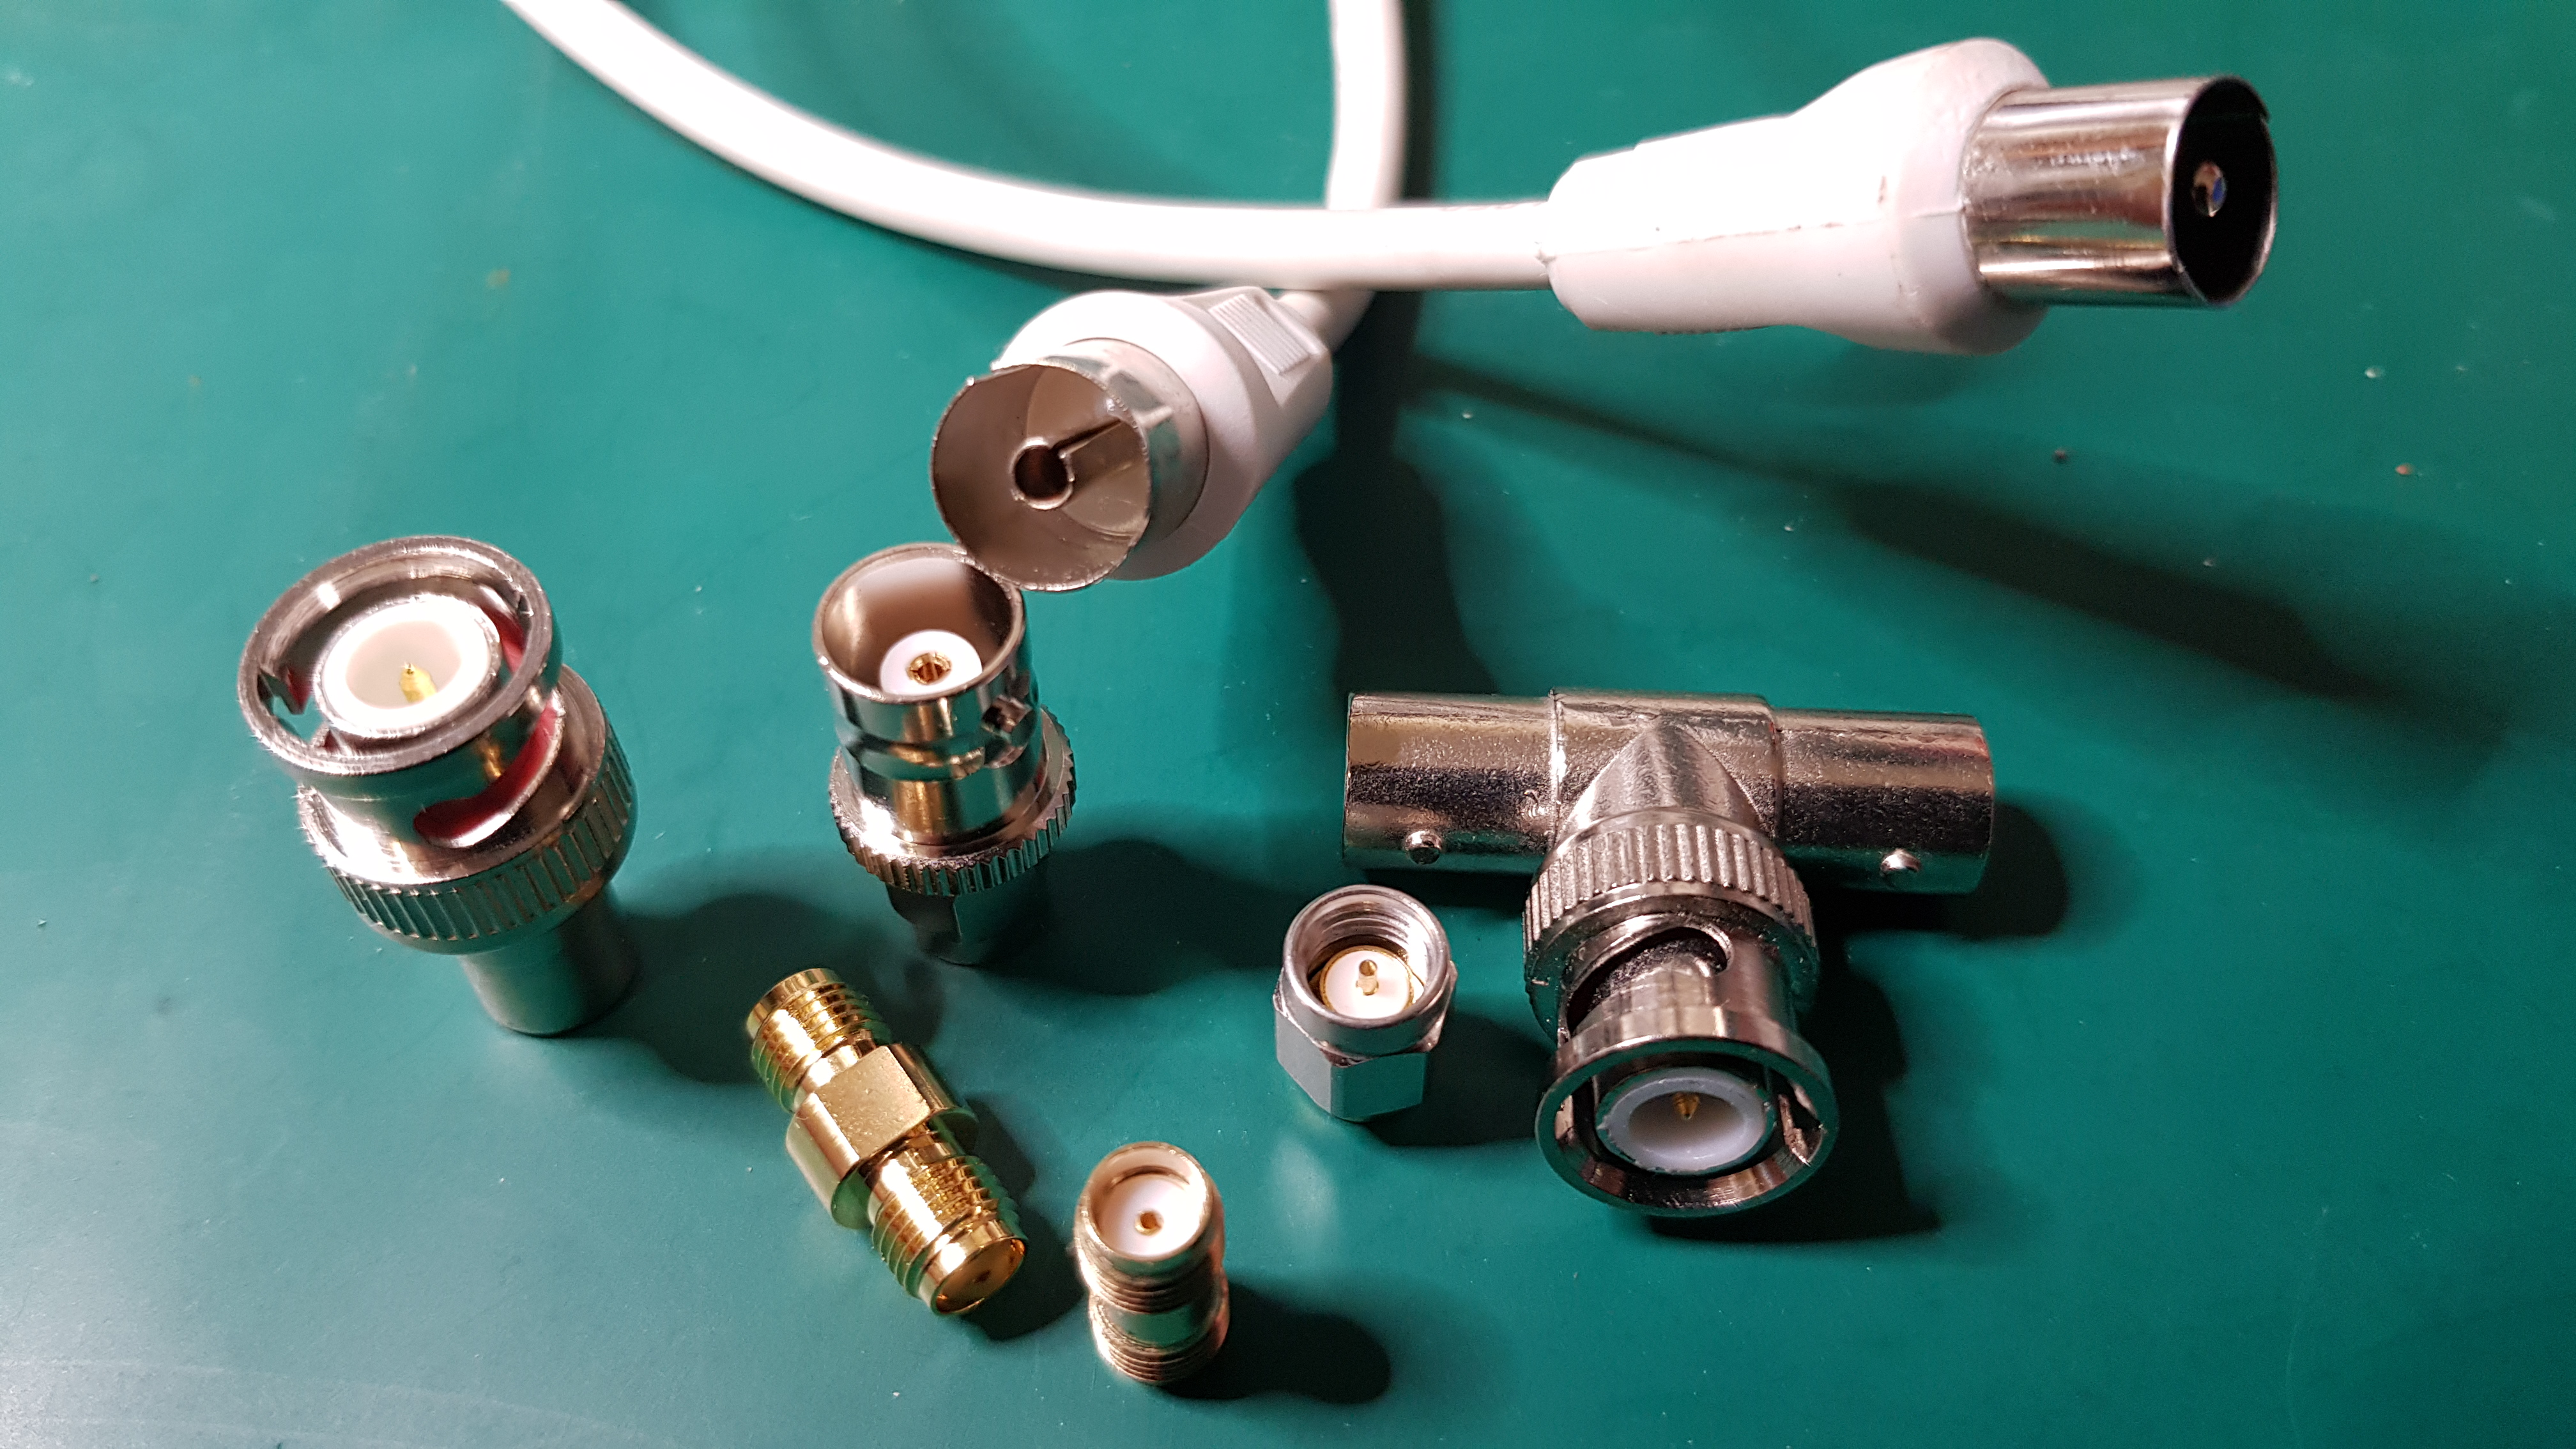
\includegraphics[width=0.65\linewidth]{coaxial_con.jpg}
  } 
  \end{column}
\end{columns}
\end{frame}

\begin{frame}{Reflections}
\begin{itemize}
 \item Improper \hyperlink{impedance_matching}{impedance matching} causes reflections
 \item Square waves include high frequency components and
       the frequency specific properties of the transmission line will distord the signal
 \item Cases: Open (reflection back), Closed (inverse reflection) - attenuation
\end{itemize}
\end{frame}

\begin{frame}[label=impedance_matching]{Impedance matching}
\begin{itemize}
 \item Required for the maximal power transfer
 \item Lossy matching can be achieved with a resistive network (often an L pad)
  \begin{itemize}
   \item Frequency independent
   \item Reactive impedance need to be insignificantly low
  \end{itemize}
 \item Reactive matching is more efficient
  \begin{itemize}
   \item Frequency specific solution with a limited bandwith
   \item Impedance matching transformermers
   \item Low pass, high pass, or bandpass configurations
  \end{itemize}
\end{itemize}
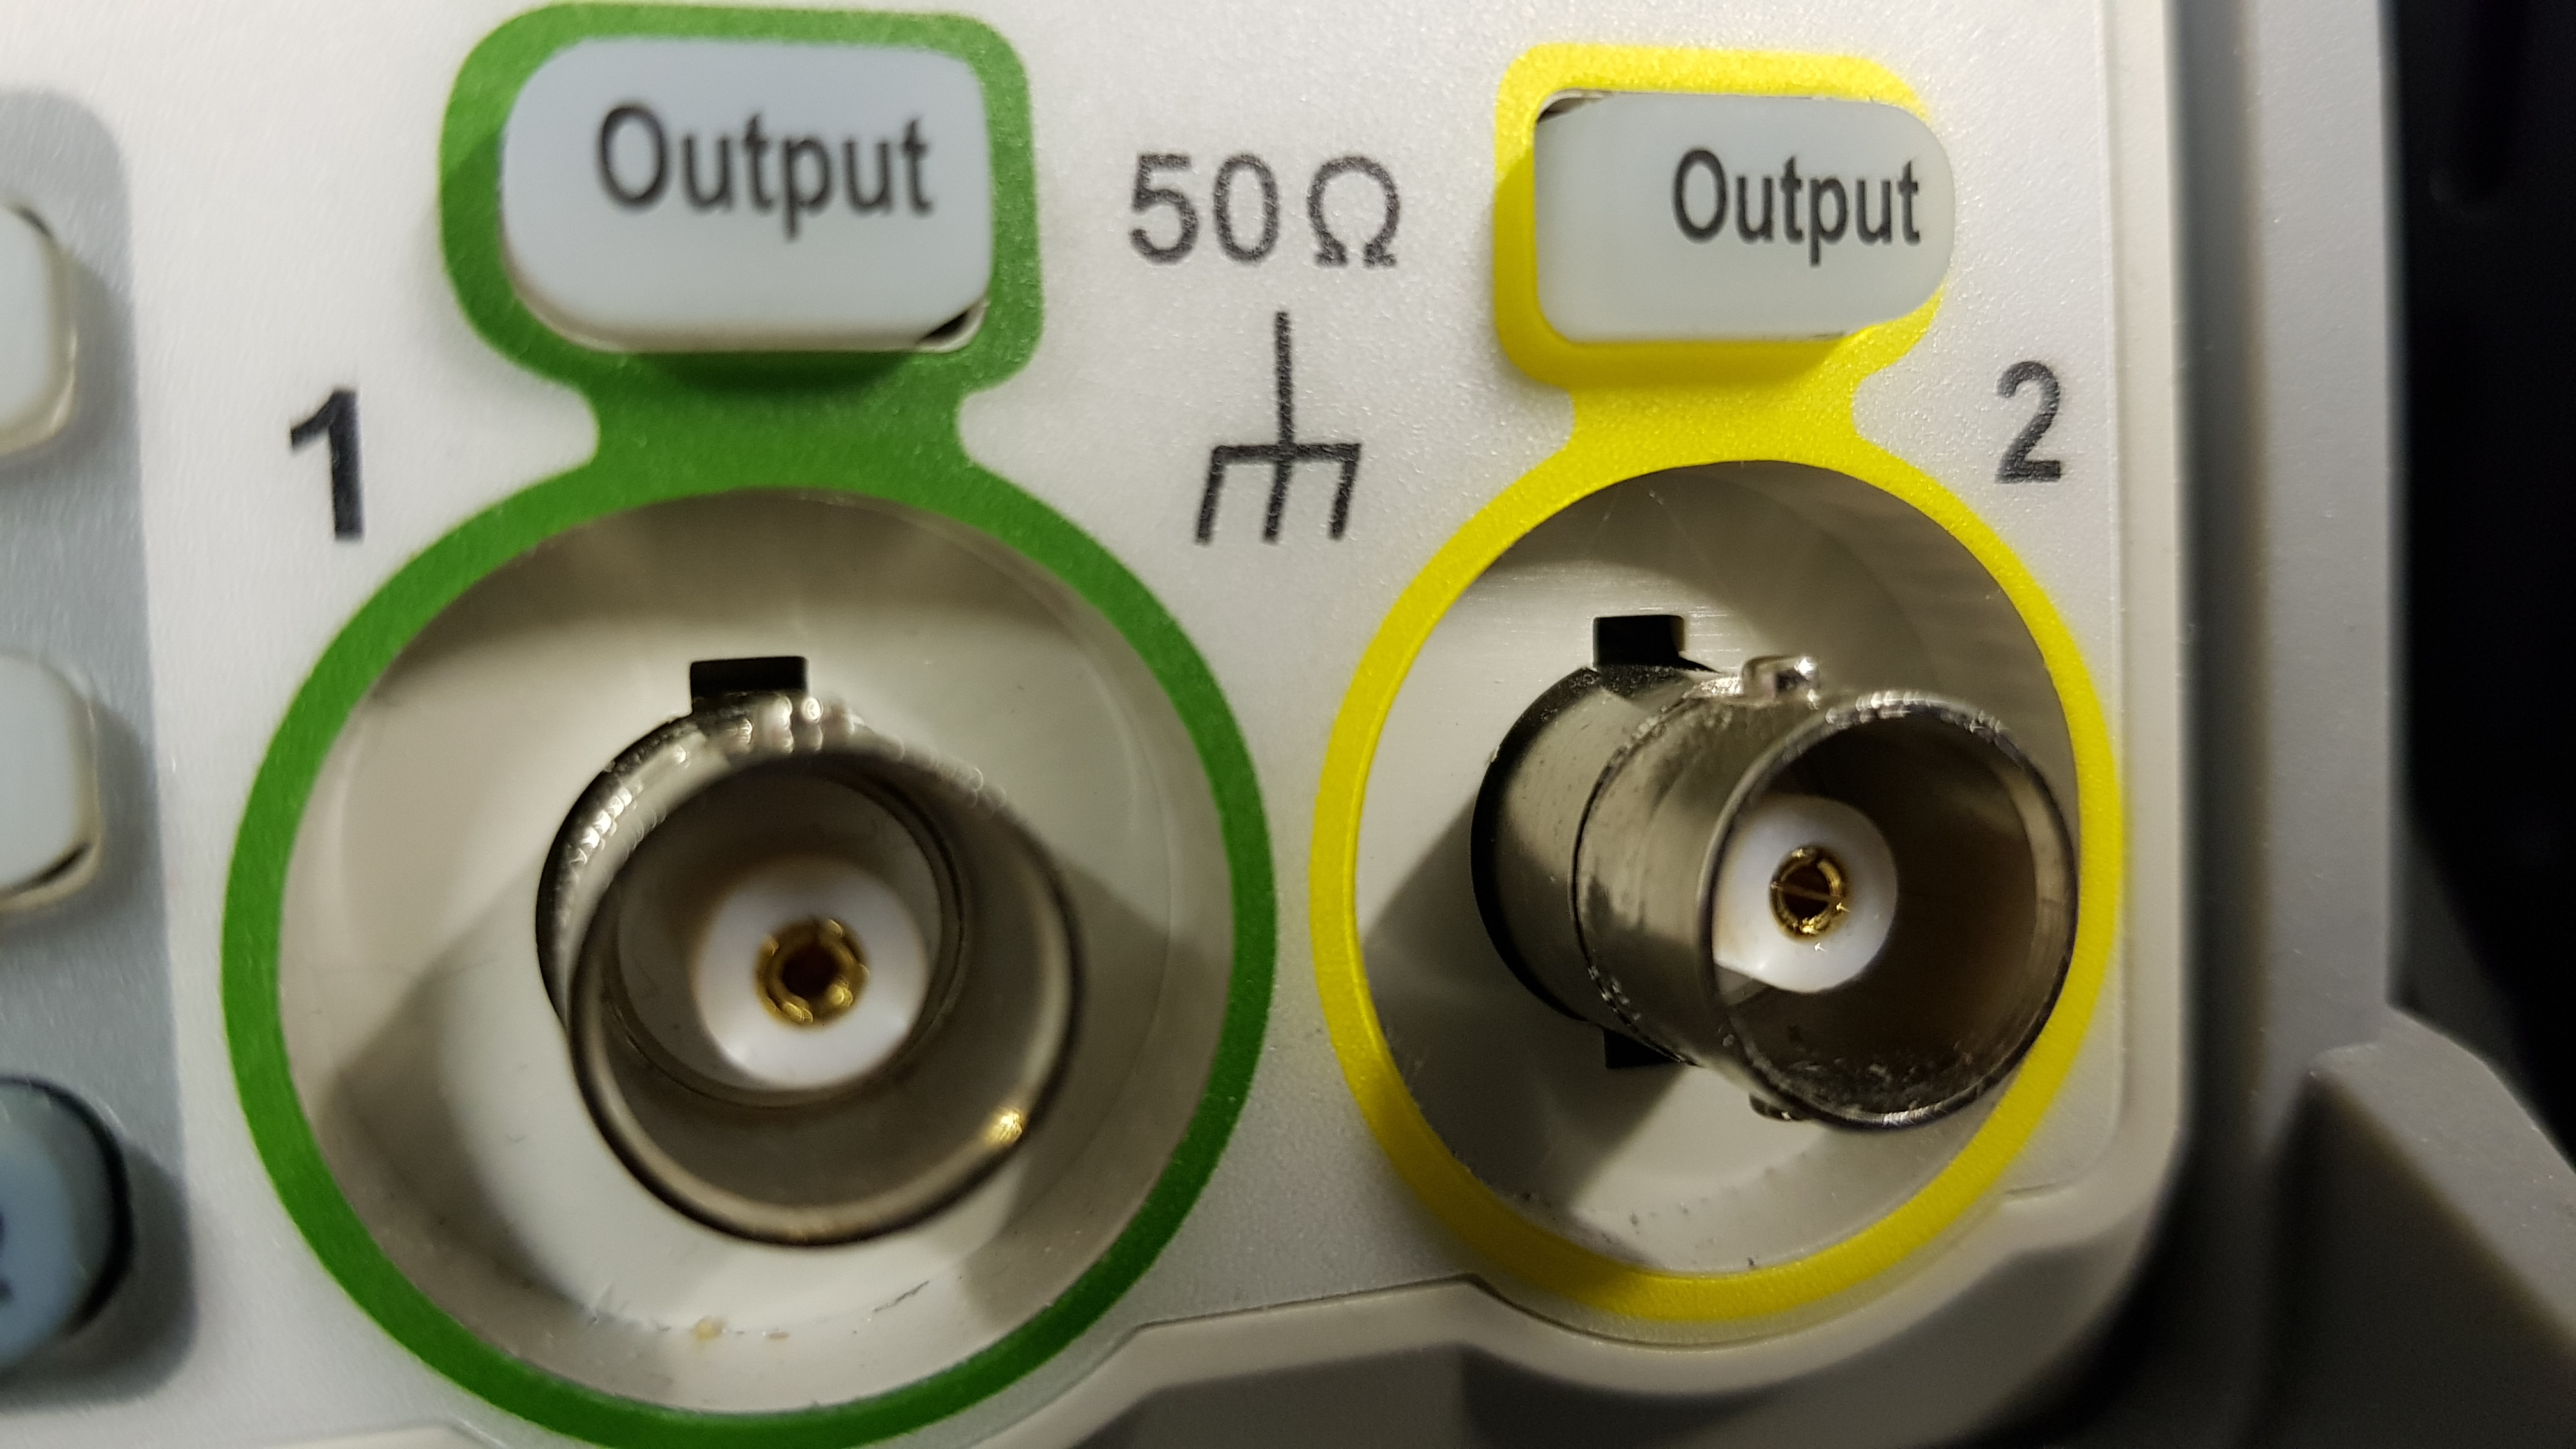
\includegraphics[width=0.4\linewidth]{coaxial_out.jpg}
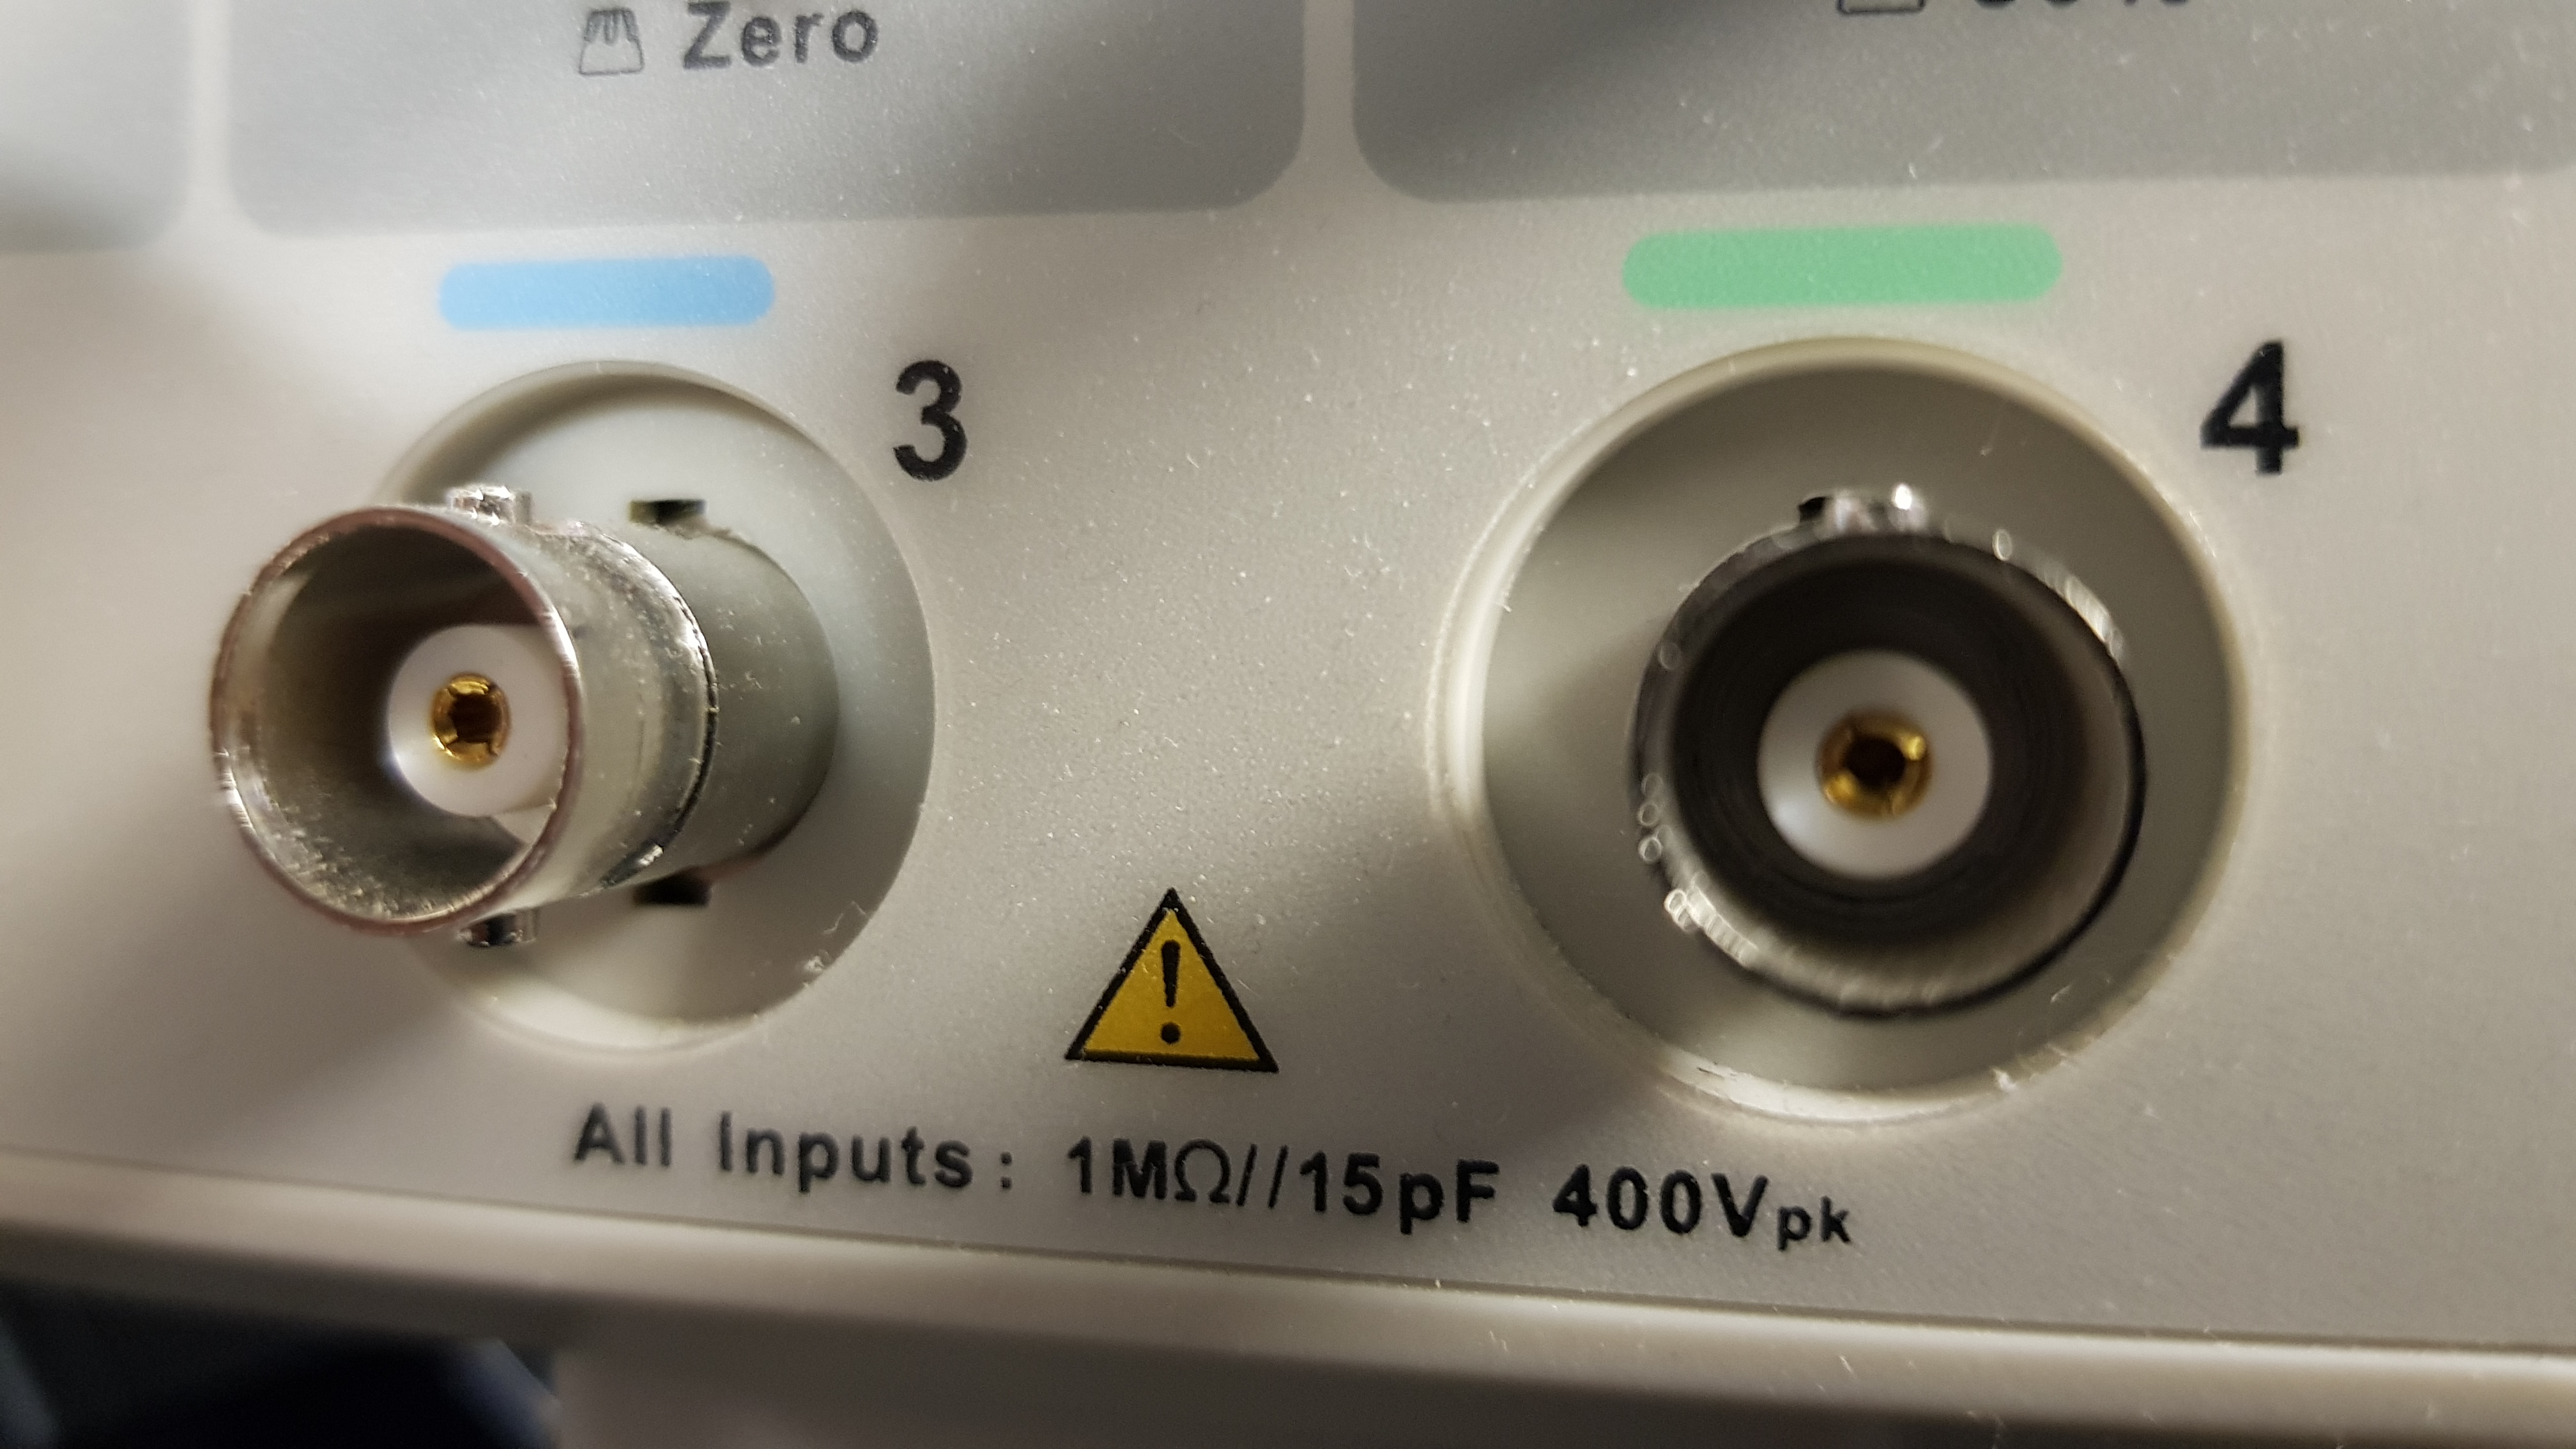
\includegraphics[width=0.4\linewidth]{coaxial_in.jpg}
\end{frame}

\begin{frame}{Termination}
\begin{columns}
  \begin{column}{0.48\textwidth}
   \begin{itemize}
    \item Terminators are used to prevent reflections
    \item Used in the end of a transmission line when the impedance of
          the load is above the transmission line
    \item Simple resistors in parallel to the load
    \item Properly terminated transmission line behave like a pure resistive loads without capacitance
   \end{itemize}
  \end{column}
  \begin{column}{0.48\textwidth}
   \tcbox[colframe=green!30!black, colback=green!30]{
    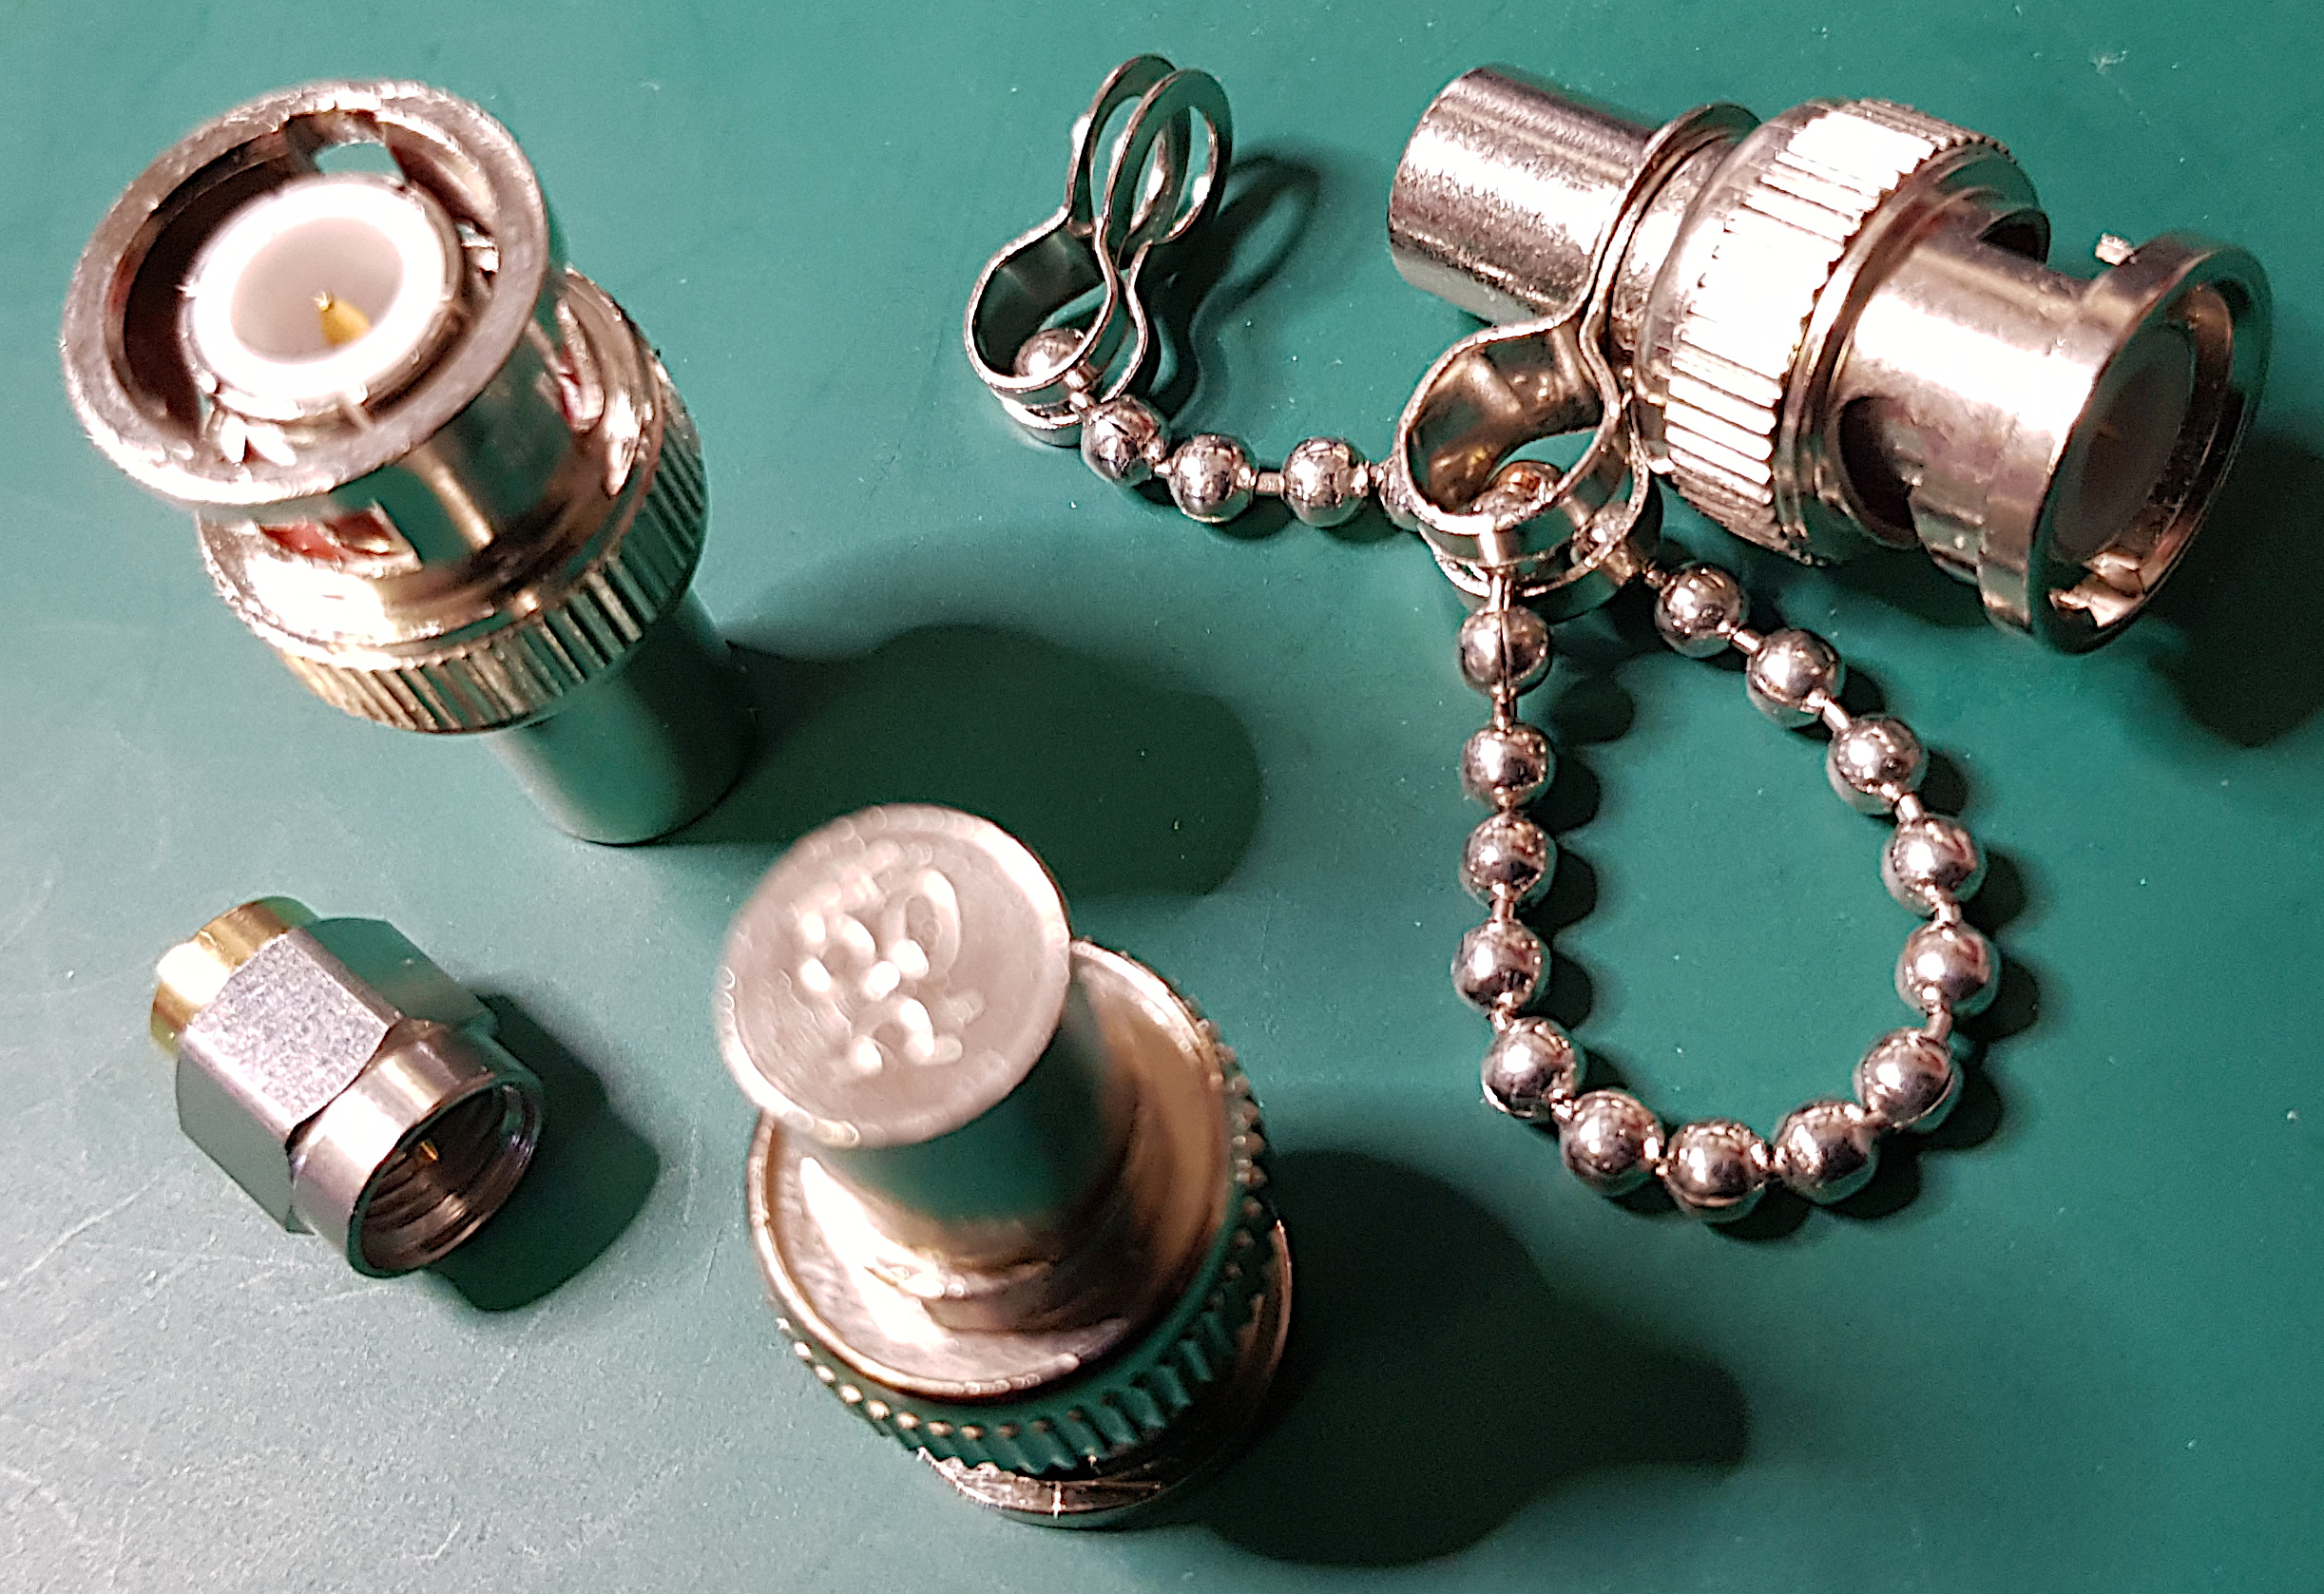
\includegraphics[width=0.65\linewidth]{terminators.jpg}
  } 
  \end{column}
\end{columns}
\end{frame}

\section{Testing reflections}

\begin{frame}{Testing reflections in practice}
\begin{itemize}
 \item Take a long cable for a reasonable delay between the test pulse and its reflection
 \item Connect your cable to a signal generator, which generates short pulses with reasonable voltages
 \begin{itemize}
  \item We are using $\SI{32.6}{\nano\second}$ pulses of $\SI{6}{\volt}$ peak-to-peak
  \item The other end of the cable is left open for the following experiments
 \end{itemize}
 \item Connect an oscilloscope probe to the input side of the cable and use input pulses for the triggering
\end{itemize}
\centering\tcbox[colframe=green!30!black, colback=green!30]{
  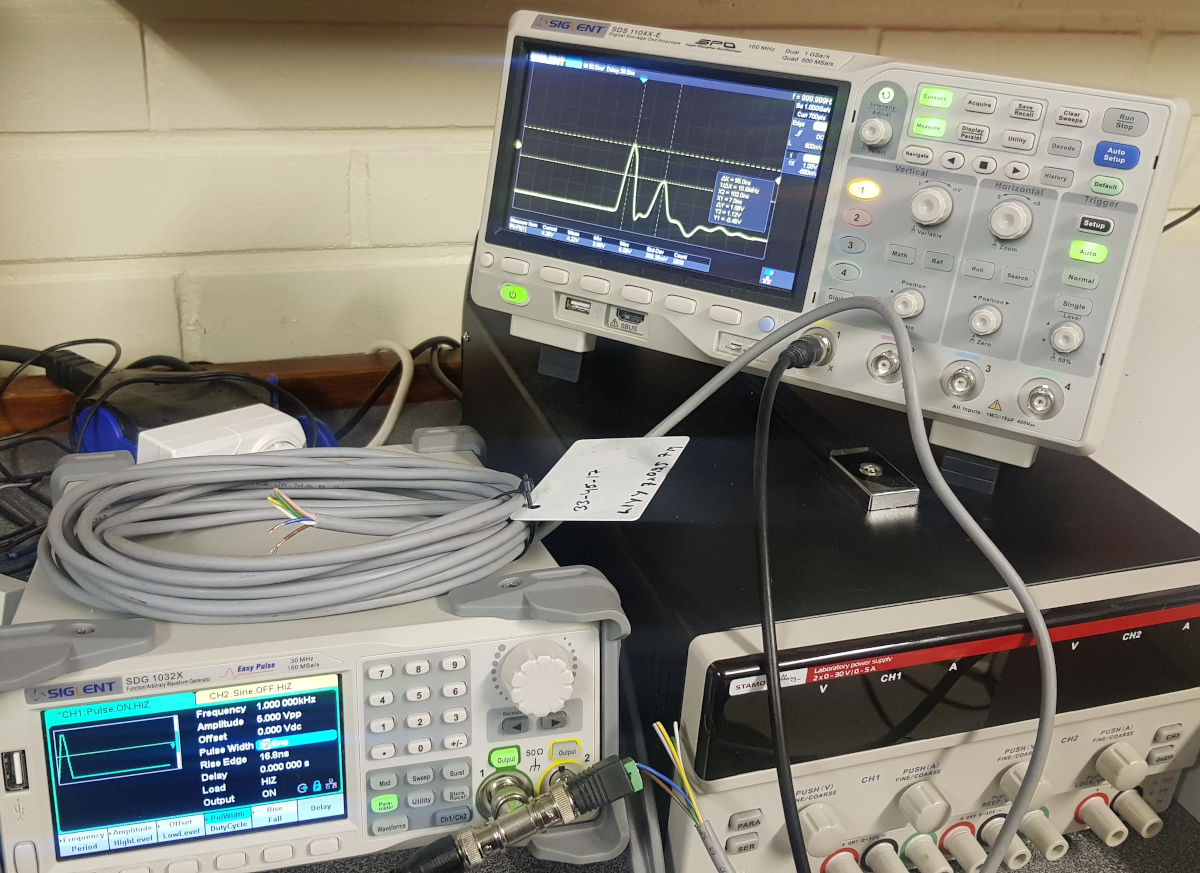
\includegraphics[width=0.30\linewidth]{pulse_setup.jpg}
}
\end{frame}

\begin{frame}{Pulse example: the setup}
\centering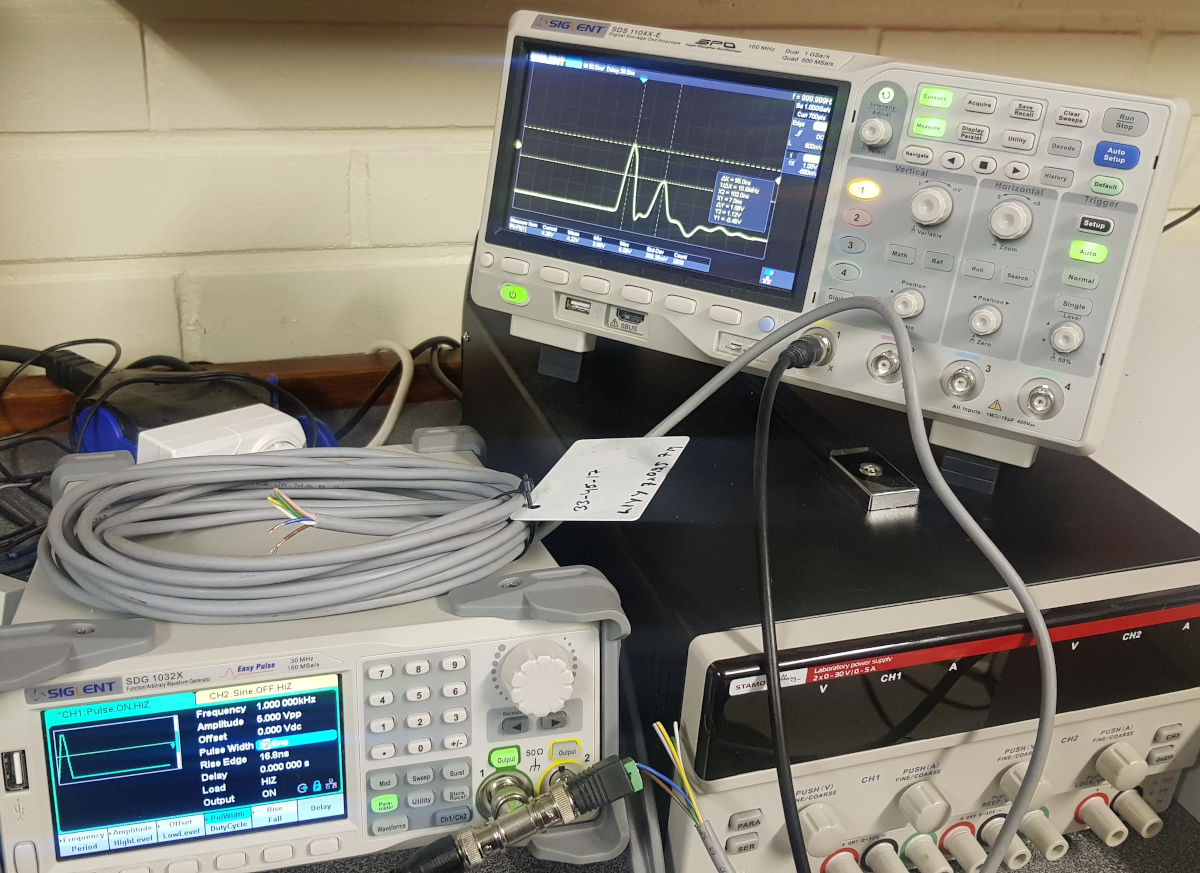
\includegraphics[keepaspectratio, width=0.75\paperwidth]{pulse_setup.jpg}
\end{frame}

\begin{frame}{Pulse example: open circuit}
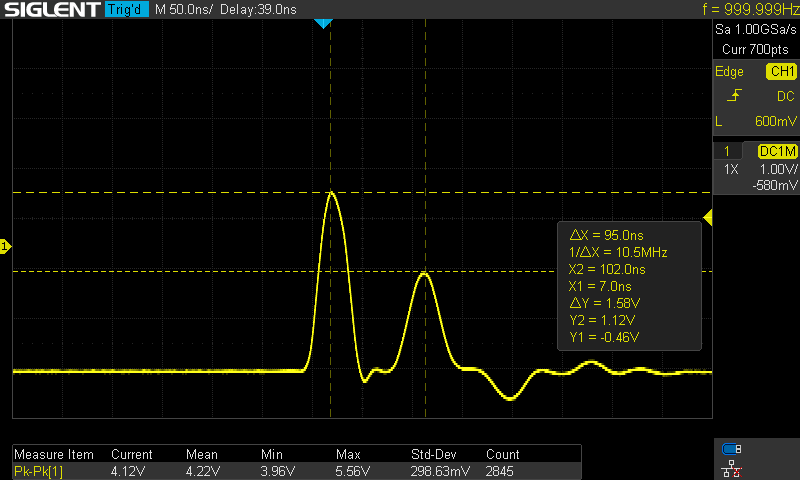
\includegraphics[keepaspectratio, width=0.85\paperwidth]{pulse_open.png}
\begin{picture}(1,1)
  \put(-313,109){\hbox{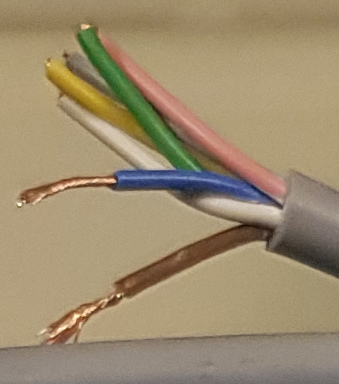
\includegraphics[scale=0.2]{pulse_disjoint.jpg}}}
\end{picture}
\end{frame}

\begin{frame}{Pulse example: closed circuit}
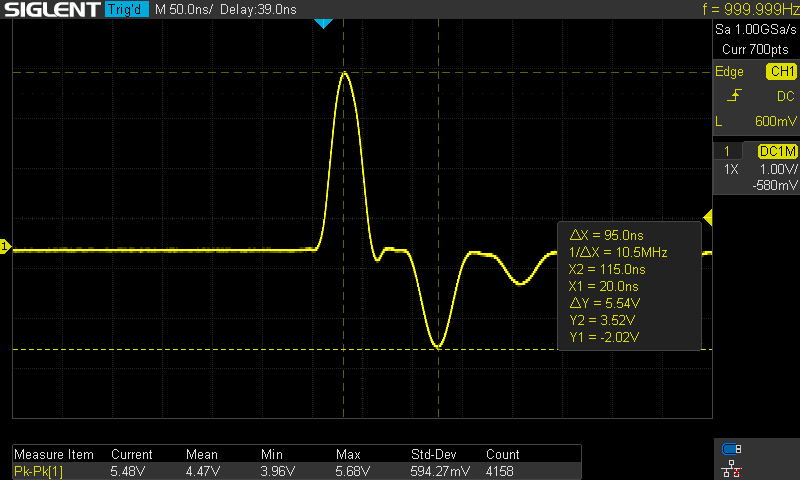
\includegraphics[keepaspectratio, width=0.85\paperwidth]{pulse_closed.png}
\begin{picture}(1,1)
  \put(-313,116){\hbox{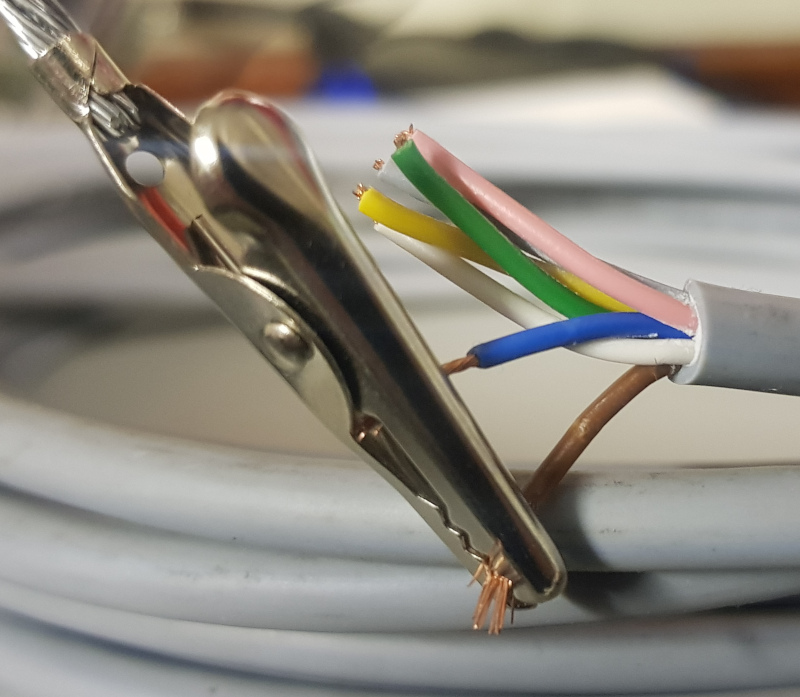
\includegraphics[scale=0.1]{pulse_short.jpg}}}
\end{picture}
\end{frame}

\begin{frame}{Pulse example: terminated circuit}
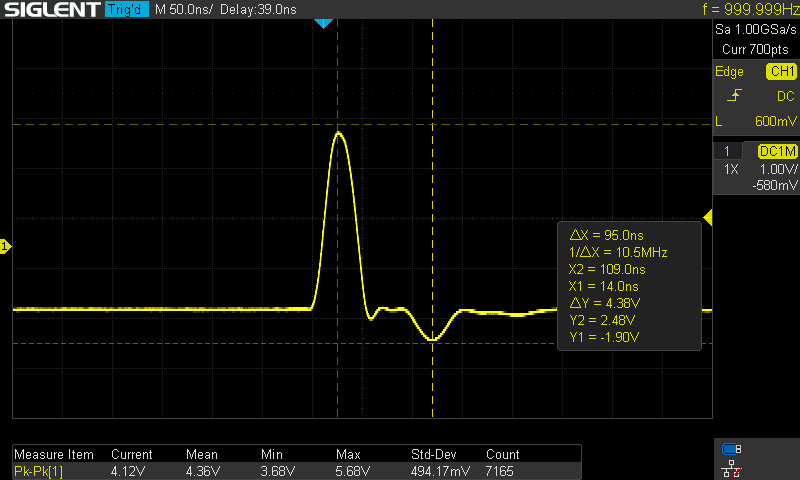
\includegraphics[keepaspectratio, width=0.85\paperwidth]{pulse_terminated.png}
\begin{picture}(1,1)
  \put(-313,87){\hbox{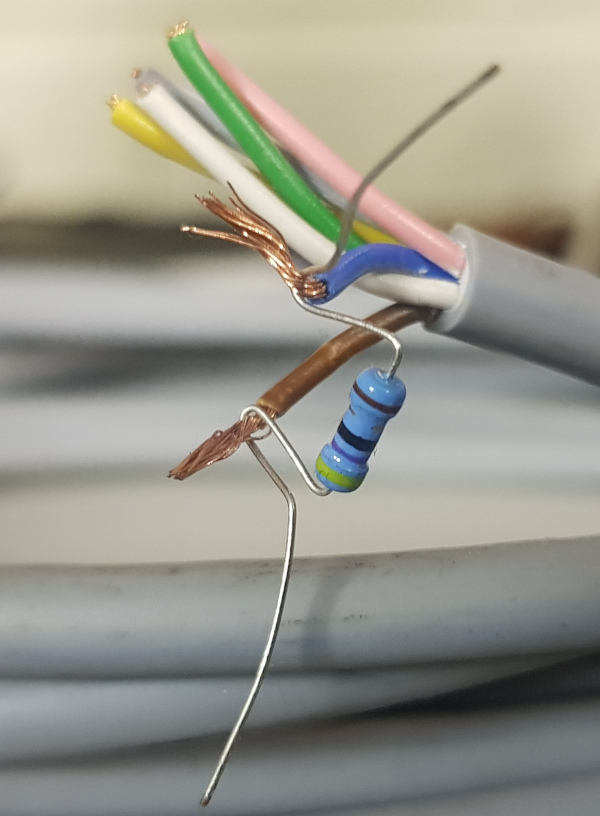
\includegraphics[scale=0.12]{pulse_resistor.jpg}}}
\end{picture}
\end{frame}

\logo{} % Disable logo
\pgfdeclareimage[width=\paperwidth]{bg}{powerline_v.jpg}
\setbeamertemplate{background}{\transparent{0.35}\pgfuseimage{bg}}
\section{References}

\begin{frame}{That's all for now}
\centering \Huge
\emph{Thank you!}
\end{frame}

\begin{frame}[t, allowframebreaks]
\frametitle{References}
\bibliographystyle{plain}
\bibliography{cable}
\end{frame}

\end{document}
